\begin{abstract}
The abstract should summarize the contents of the paper.
It should be clear, descriptive, self-explanatory and not longer
than 200 words. It should also be suitable for publication in
abstracting services. Please avoid using math formulas as much as possible.

This is a sample input file.  Comparing it with the output it
generates can show you how to produce a simple document of
your own.
\end{abstract}

%% \begin{keyword}[class=MSC]
%% \kwd[Primary ]{60K35}
%% \kwd{60K35}
%% \kwd[; secondary ]{60K35}
%% \end{keyword}

%% \begin{keyword}
%% \kwd{sample}
%% \kwd{\LaTeXe}
%% \end{keyword}

\section{Introduction}
Since the seminal papers by Bollerslev~\cite{bollerslev:1986} and 
Taylor~\cite{taylor:2008} (cf. also Andersen et al
\cite{andersen:davis:kreiss:mikosch:2009}), the GARCH 
({\em Generalized Autoregressive Conditional Heteroscedasticity}) model
has been widely used in finance and economics, and has
inspired numerous variants such as GJR-GARCH of Glosten et
al~\cite{glosten:1993}, {\em Asymmetric} GARCH of Engle and
Ng~\cite{engle:Ng:1993} and the {\em Quadratic} GARCH of
Sentana~\cite{sentana:1995}, among others. The basic GARCH model of
Bollerslev~\cite{bollerslev:1986} and Taylor~\cite{taylor:2008}
defines the conditional variance via the stochastic recurrence
equation
\begin{eqnarray}
  R_t &=& \sigma_t Z_t \nonumber \\
  \sigma_{t}^2 &=& \omega + \sum_{i=1}^p \alpha_i R_{t-i}^2 +
  \sum_{j=1}^q \beta_j \sigma_{t-j}^2   \label{eq:garchpq}
\end{eqnarray}
where $\{R_t\}_{t \in \mathbb Z}$ is the return series in question;
$\{Z_t\}_{t \in \mathbb Z}$ is an iid sequence of random variables
with zero mean and unit variance; the distribution function of $Z_t$
is assumed to have a density.
$\omega, \alpha_i, i \in \{1,\dots,p\}$ and
$\beta_j, j \in \{1,\dots,q\}$ are constant parameters. A process
defined by \eqref{eq:garchpq} is called a GARCH($p,q$) process.
When $p = q = 1$,
\[
\sigma_t^2 = \omega + (\alpha_1 Z_{t-1}^2 + \beta_1) \sigma_{t-1}^2
\]
When $p > 1$ or $q > 1$, the GARCH($p, q$) process is given by
a matrix recurrence equation (cf. Davis and
Mikosch~\cite{davis:mikosch:2001}).
Define $d = p + q - 1$ and we can write the recurrence equation as
\begin{equation}
  \label{eq:garchpq_sre}
  V_t = A_t V_{t-1} + B_t
\end{equation}
where $V_t$ and $B_t$ are $d$-dimensional vectors; $A_t$ are
$d \times d$ matrices. The sequences $A_t$ and $B_t$ are both iid.
Of course, $B_t$ are really constant vectors, but we postpone this
specialization for now and generalize the equation
\eqref{eq:garchpq_sre} to the broader context of matrix recursions.
There is already a rich literature on this subject. Kesten
\cite{kesten:1973} showed that, when $A_t$ and $B_t$ were almost
surely non-negative, had no row or column of only zeros, and there was
a positive probability that $B_t$ was strictly positive, the strictly
stationary solution to the equation
$V \overset{d}{=} A V + B$ had power-law tails
for its marginal distributions, assuming the following conditions (M)
and (A):
\begin{itemize}
\item Condition (M)
  \begin{enumerate}
  \item The top Lyapunov exponent
    \[
    \gamma = \inf_{n \geq 1} {1 \over n}\E \log \|A_n \cdots A_1\|
    \]
    is negative.
  \item There exists $\xi > 0$ such that
    \[
    1 = \lambda(\xi) = \lim_{n \to \infty} {1 \over n} \log \E \|A_n \cdots A_1\|^\xi
    \]
  \item $\E (\|A_1\|^\xi \log^+\|A_1\|) < \infty$
  \item $\E |B_1|^\xi < \infty$
  \end{enumerate}
\item Condition (A) : The group generated by
  \[
  \{\log\rho(s): s = A_n \cdots A_1 \text{ for some } n \geq 1\}
  \]
  is dense in $\reals$, where $\rho(s)$ denotes the spectral
  radius of matrix $s$.
\end{itemize}
Upon these conditions, Kesten's theorem gives
\begin{equation}
  \label{eq:kesten}
  u^\xi \P(u^{-1} V \in \cdot) \overset{v}{\to} \mu_\xi(\cdot)
\end{equation}
where $\mu_\xi$ is a non-null Radon measure on
$\reals^d_+ \setminus \{0\}$ with the property
$\mu_\xi(a A) = a^{-\xi} \mu_\xi(A)$.

Recently, Collamore and Mentemeier \cite{collamore:mentemeier:2016}
extended Kesten's result and gave an explicit expression for $\mu_\xi$:
\begin{equation}
  \label{eq:CollamoreMentemeier}
  \lim_{u \to \infty} u^{\xi} \E \left[
    f(u^{-1} V)
    \right]
  =
  {C \over \lambda'(\xi)}  
  \int_{\sphere^{d-1}_+ \times \reals} e^{-\xi s} f(e^s x) \ell_\xi(dx) ds
\end{equation}
where $C$ is a constant (cf. eq.(2.15) of Collamore and Mentemeier
\cite{collamore:mentemeier:2016}), $f(\cdot)$ is any bounded
continuous function on $\reals^{d}_+ \setminus \{0\}$  and
$\ell_\xi$ is a probability measure on $\sphere_+^{d-1}$. Its definition
is also found in \eqref{eq:eigenmeasure}.

From \eqref{eq:CollamoreMentemeier} a representation for
$\mu_\xi (\cdot)$ immediately follows 
\[
\mu_\xi (\cdot) = {C \over \lambda'(\xi)} \mathcal L_\xi(\cdot)
\]
Here $\mathcal L_\xi$ is a non-null Radon measure  on
$\reals^d_+ \setminus \{0\}$ that satisfies, for all
bounded continuous function $f(\cdot)$ on
$\reals_+^{d} \setminus \{0\}$:
\[
\int_{\reals_+^d\setminus \{0\}} f(x) \mathcal L_\xi(dx)
=
\int_{\sphere^{d-1}_+ \times R} e^{-\xi s} f(e^s x) \ell_\xi(dx) ds
\]
A key ingredient of Collamore and Mentemeier's approach is Hennion's
uniform convergence result on the product of iid random matrices
\cite{hennion:1997}:
\[
\limsup_{n \to \infty}
\left\{
  {1 \over n} \1{n > T}
  \left|
  \log \inn{y, A_n \cdots A_1 x} - \gamma
  \right|
  :
  x, y \geq 0, |x| = 1, |y| = 1
  \right\} = 0
\]
where
\begin{equation}
  \label{eq:hennion_T}
  T = \min\{n \geq 1, A_n \cdots A_1 > 0\}.
\end{equation}
Conditions (I, II, III) of hypothesis \ref{hypo:1} and (ii) of remark
\ref{remark:fhrtgh} imply $T$ as defined in \eqref{eq:hennion_T} is
almost surely finite. Cf. Buraczewski et al
\cite{buraczewski:damek:mikosch:2016}, example 
  4.4.13, Kesten \cite{kesten:1973}, eq.(2.56) and Hennion
  \cite{hennion:1997}, lemma 3.1., $T$ is almost surely finite.
Here $x \geq 0$ means every component of $x$ is non-negative.

In addition to non-negative matrices, two other classes of random
matrices have been shown to lead to power-law tails via the recurrence
relation \eqref{eq:garchpq_sre}. Alsmeyer and Mentemeier
\cite{alsmeyer:mentemeier:2012} considered invertible matrices whose
distribution has a density. Let $M(d, \reals)$ denote the space of
$d \times d$ matrices with real entries that are invertible with
probability 1. They replaced Kesten's condition
$\E (\|A\|^\xi \log^+\|A\|) < \infty$ with a stronger
counterpart
$\E [\|A\|^\xi (\log^+\|A\| + \log \|A^{-1} \|)] < \infty$,
and lifted the condition (A). In addition, they assumed
\begin{enumerate}
  \item The Markov chain $X_n$ on $\sphere^{d-1}$, namely
    $X_n = A_n X_{n-1} / |A_n X_{n-1}|$, is irreducible, i.e. for any open
    set $U \subset \sphere^{d-1}$ and any $u \in \sphere^{d-1}$, 
    $\exists n \geq 1$ such that $\P(X_n u \in U) > 0$.
  \item There exist $N \geq 1$, $c, \epsilon > 0$ and an invertible
    matrix $\bar A \in M(d, \reals)$ such that for any set
    $C \subset M(d, \reals)$, it holds true
    $\P(A_N \cdots A_1 \in C) \geq c |B_\epsilon(\bar A) \cap C|$,
    where $|\cdot|$ denotes the Lebesgue measure.
\end{enumerate}
These assumptions are termed conditions (id). Furthermore, they assumed
that there was no point in $\reals^d$ such that the recurrence
equation \eqref{eq:garchpq_sre} was stuck at this point with probability 1: 
$\P(A X + B = X) < 1$ for all $X \in \reals^d$ and all $A \in M(d, \reals)$.
With these assumptions, they showed
\[
\lim_{u \to \infty} u^\xi \P(\inn{x, V} > u) = e_\xi(x)
\]
where $x \in \sphere^{d - 1}$ and $e_\xi(\cdot)$ is a continuous
function $\sphere^{d-1} \to \reals_+$.

The second of the (id) conditions, which is satisfied when the
distribution of $A$ has a Lebesgue density, can actually be lifted if
stronger moment conditions are imposed on $A$ and $B$, and in
addition, a proximity condition is satisfied by the support of
$A$. This is the result of Guivarc'h and Le Page, et al
\cite{guivarc:page:2016}. Let $G_A$ denote the semi-group generated
by $\{\Pi_n: \Pi_n = A_n \cdots A_1, A_i \in M(d, \reals)\}$. The
authors assumed
\begin{enumerate}
  \item There is no finite union $W$ of proper subspaces of $\reals^d$
    that satisfies $\forall a \in G_A, a W = W$.
  \item $G_A$ contains a proximal element, i.e. an element $a$ whose
    largest singular value is an algebraically simple eigenvalue of $a$.
\end{enumerate}
These two assumptions are termed (ip) conditions. Replacing the (id)
conditions of Alsmeyer and Mentemeier with (ip) and the moment
conditions of the former with
\[
\E \|A\|^{\xi + \delta} < \infty, \quad
\E (\|A\|^{\xi} \|A^{-1}\|^{\delta}) < \infty, \quad
\E (|B|^{\xi + \delta} < \infty),\quad
\text{ for some }\delta > 0
\]
Guivarc'h and Le Page et al proved the same vague convergence result
of \eqref{eq:kesten}.

In the special case of GARCH($p, q$),
Bollerslev \cite{bollerslev:1986} showed that the 
equation $X \overset{d}{=} A X + B$ has a unique, strictly
stationary solution with finite variance if and only if
\begin{equation}
  \sum_{i=1}^p \alpha_i + \sum_{j=1}^q \beta_j < 1
  \label{eq:bollerslev}
\end{equation}
In the rest of this paper, we always assume condition
\eqref{eq:bollerslev} is satisfied. For convenience of narration, let
$\pi$ denote this unique stationary probability measure and let
$V \sim \pi$, $Z \sim \mu_Z$. More generally we write $\mu_U$ for the
probability measure of $U$, no matter what type of object $U$ may be.

Buraczewski et al \cite{buraczewski:damek:mikosch:2016} (proposition
4.3.1) derived the support of $\pi$ assuming the condition of
Bollerslev \ref{eq:bollerslev}. We omit the formula here and refer to it as
$\chi$ hereafter.

%% According to Buraczewski et al 
%% \cite{buraczewski:damek:mikosch:2016}, proposition 4.3.1, the support
%% of $\pi$ is
%% \[
%% \chi = \overline{
%%   \left\{
%%   (I_{p+q-1} - a)^{-1} b:
%%   \exists n \geq 1,
%%   a = \prod_{i=1}^n A_i,
%%   \|a\| < 1,
%%   b = \left(\sum_{i=0}^{n-1} \prod_{j=1}^i A_{j}\right) B,
%%   \right\}
%% }
%% \]
%% where $I_{\cdot}$ denotes the $\cdot \times \cdot$ identity matrix and
%% $\overline S$ denotes the closure of set $S$.

In addition to \eqref{eq:bollerslev}, we assume:
\begin{hypothesis}
  All the following conditions hold:
  \label{hypo:1}
  \begin{enumerate}[(I)]
  \item $\exists s > 0$ such that
    $1 < \E (\alpha_1 Z^2 + \beta_1)^s < \infty$
  \item If $p, q \geq 2$, there exists an non-empty open set
    $S \subset \supp \mu_Z$.
  \item $\alpha_p > 0$  and $\beta_q > 0$.
  \end{enumerate}
\end{hypothesis}
Clearly, these conditions are satisfied when $Z$ has normal or $t$
distributions.
\begin{remark}
  \label{remark:fhrtgh}
  From hypothesis \ref{hypo:1}, a few implications immediately follow
  \begin{enumerate}[(i)]
  \item \eqref{eq:garchpq} implies
    \[
    \sigma_t^2 \geq \omega \left(
      1 - \sum_{j=1}^q \beta_j
    \right)^{-1} = \sigma_{\m}^2 > 0
    \]
    Then it follows
    $\chi \subseteq [\sigma_{\m}^2, \infty)^q \times [0, \infty)^{p-1}$, so
    $V_n \in \chi$ for all $n \geq 0$. Since the random variable
    $Z_{n-1}^2$ is assumed to have a continuously differentiable
    distribution function,
    $\P(Z_{n-1}^2 = x) = 0$ for all $x \in \text{supp } \mu_{Z^2}$.
    Furthermore, $Z_{n-1}^2$ uniquely determines the matrix $A_n$,
    so it follows $\P(A v + B = v) = 0$ for all $v \in \chi$.
  \item \eqref{eq:bollerslev} implies the top Lyapunov exponent of $A_n$
    \begin{equation}
      \label{eq:Lyapunov}
      \gamma = \inf_{n \geq 1} {1 \over n}
      \E \left(\log \| A_n \cdots A_1 \| \right)    
    \end{equation}
    is negative. Cf. Buraczewski et al
    \cite{buraczewski:damek:mikosch:2016}, prop. 4.1.12.

  \item That $\vec 0 \notin \chi$ and $A_n$ has a Lebesgue density
    implies the stationary distribution $\pi$ is absolutely continuous with
    respect to Lebesgue measure. This immediately follows from lemma
    4.2.2 of Buraczewski et al \cite{buraczewski:damek:mikosch:2016}.

  \item Condition (III) ensures that, with probability 1, every row and
    column of the matrix $A_n$ has at least one postive component.
  \end{enumerate}
\end{remark}
The implications (i), (ii), (iii) are in fact the conditions of
proposition 4.2.1 of Buraczewski et al
\cite{buraczewski:damek:mikosch:2016}, from which we conclude $V_n$ is
an aperiodic, positive Harris chain that is in addition
$\pi$-irreducible on $\chi$.
Moreover, from (I) it follows $0 < \exists \xi < s$ such that
\begin{equation}
  \label{eq:hyt}
  \lambda(\xi) = \lim_{n \to \infty} (\E \|A_n \cdots A_1\|^\xi)^{1/n} = 1
\end{equation}
and
\begin{equation}
  \label{eq:jui}
  \E \|A\|^\xi < \infty
\end{equation}
The existence of $\xi$ together with Conditions (ii, iv) and (I, II)
allow the application of Kesten's theorem (cf. Buraczewski et al
\cite{buraczewski:damek:mikosch:2016}, example 4.4.13).
% Here and in the rest of this paper, we use $\tilde V$ to denote $V/|V|$, $V'$ to
% denote the transpose of $V$ for a vector $V$,
% and $\tilde S$ to denote $\{\tilde v: v \in S\}$ for a set $S$.
% The Kesten's theorem gives
% \begin{equation}
%   \label{eq:kesten}
%   \lim_{x \to \infty} x^{\xi} \P(\tilde y' V > u) = e_\xi(\tilde y)  
% \end{equation}
% for some function $e_\xi: \tilde \chi \to \reals_+$ and
% all $\tilde y \in \tilde \chi$. Here $d = p + q - 1$.
% Cf. Kesten
% \cite{kesten:1973} and  Buraczewski et al
% \cite{buraczewski:damek:mikosch:2016},
% section 4.4.4.

Although the probability $\P(\inn{\tilde x, y} > u)$ has been given
asymptotically by Kesten's theorem, one often wishes to know
this probability more precisely, due to the importance of risk
management. Now that more detailed analytic description of the
probability is unknown, one has to resort to numerical methods. But
the occurrence of $\inn{\tilde x, V} > u$ for a large $u$ is a rare event; a
naive Monte-Carlo approach will be very inefficient. Cf. Asmussen and
Glynn \cite{opac-b1123521}.
One way to increase the efficiency of Monte-Carlo methods is
importance sampling.

%TODO: Add literature review of importance sampling%
% Jose Blanchet & Peter Glynn: Annals of appl. prob. 2008
The idea of importance sampling with exponential shift dates back
to Siegmund \cite{siegmund:1976}, who devised an algorithm for
estimating the excursion probability of 1D random walk with iid
increments. Following his work, various importance sampling algorithms
have been proposed for rare event simulation in a variety of problems.

Let $W_n = \sum_{i=1}^n X_n$ be a random walk. Blanchet and Glynn
\cite{blanchet:glynn:2008}
proposed a state-dependent importance sampling algorithm to estimate
the tail of $\max\{W_n, n \geq 1\}$ and showed that their estimator
had bounded relative error (cf. Asmussen and Glynn
\cite{opac-b1123521}). In the case of light tailed increments, their
estimator recovers that of Siegmund.

In 2010, Blanchet and Liu \cite{blanchet:liu:2010} presented an
importance sampling algorithm for the first passage time of a
multidimensional random walk with heavy-tailed increments.

However, to our best knowledge, no importance sampling
estimator has been proposed in the literature for the computation of
$\P(\inn{\tilde x, V} > u)$ or for the more general problem when the
defining recurrence equation of $V_n$ i.e. \eqref{eq:garchpq_sre} is 
more general than that of GARCH($p, q$). We present a solution in this
paper.

When $p = q = 1$, $V_n$ reduces to a scalar. An importance sampling
estimator was proposed and shown to be efficient in the sense of
bounded relative error by Collamore et al \cite{collamore2014}. We
consider our work as a multivariate extension to theirs.

\section{Statement of Results}
Our solution involves associating a {\em Markov Additive} process
$(X_n, S_n)$ to the Markov chain $V_n$:
\begin{eqnarray}
X_t &=& {
        A_t A_{t-1} \cdots A_1 \tilde V_0
        \over
        |A_t A_{t-1} \cdots A_1 \tilde V_0|
      }, \quad X_0 = \tilde V_0 \label{eq:X_def}\\
S_t &=& \log |A_t \cdots A_1 \tilde V_0| \label{eq:S_def}\\
\l_t &=& S_t - S_{t-1} = \log |A_t X_{t-1}| \label{l_def}
\end{eqnarray}
where $\tilde v = v/|v|$  for a vector $v$. From the GARCH($p, q$)
recurrence relation
\begin{tiny}
  \begin{equation*}
      \begin{pmatrix}
        \sigma_{t}^2 \\
        \sigma_{t-1}^2 \\
        \vdots \\
        \sigma_{t-q+2}^2 \\
        \sigma_{t-q+1}^2 \\
        R_{t-1}^2 \\
        R_{t-2}^2 \\
        \vdots \\
        R_{t-p+2}^2 \\
        R_{t-p+1}^2
      \end{pmatrix}
      =
      \begin{pmatrix}
        \alpha_1 Z_{t-1}^2 + \beta_1 & \beta_2 & \cdots &
        \beta_{q-1} & \beta_q & \alpha_2 & \alpha_3 &
        \cdots & \alpha_{p-1} & \alpha_p\\
        1 & 0 & \cdots & 
        0 & 0 & 0 & 0 & \cdots & 0 & 0 \\
        \vdots & \vdots & \ddots & 
        \vdots & \vdots & \vdots & \vdots &
        \ddots & \vdots & \vdots \\
        0 & 0 & \cdots &
        0 & 0 & 0 & 0 & \cdots & 0 & 0 \\
        0 & 0 & \cdots &
        1 & 0 & 0 & 0 & \cdots & 0 & 0 \\
        Z_{t-1}^2 & 0 & \cdots &
        0 & 0 & 0 & 0 & \cdots & 0 & 0 \\
        0 & 0 & \cdots &
        0 & 0 & 1 & 0 & \cdots & 0 & 0 \\
        \vdots & \vdots & \ddots &
        \vdots & \vdots & \vdots & \vdots &
        \ddots & \vdots & \vdots \\
        0 & 0 & \cdots &
        0 & 0 & 0 & 0 & \cdots & 0 & 0 \\    
        0 & 0 & \cdots &
        0 & 0 & 0 & 0 & \cdots & 1 & 0 \\    
      \end{pmatrix}
      \begin{pmatrix}
        \sigma_{t-1}^2 \\
        \sigma_{t-2}^2 \\
        \vdots \\
        \sigma_{t-q+1}^2 \\
        \sigma_{t-q}^2 \\
        R_{t-2}^2 \\
        R_{t-3}^2 \\
        \vdots \\
        R_{t-p+1}^2 \\
        R_{t-p}^2
      \end{pmatrix}
      +
      \begin{pmatrix}
        \omega \\
        0 \\
        \vdots \\
        0 \\
        0 \\
        0 \\
        0 \\
        \vdots \\
        0 \\
        0 \\
      \end{pmatrix}
  \end{equation*}
\end{tiny}
it is obvious that, by define mapping
\[
g: (x, y, l) \in \sphere^{d-1} \times \sphere^{d-1} \times \reals
\to
\reals_+ \ni {
  \inn{\vec e_{q+1}, e^l y}
  \over
  \inn{\vec e_{1}, x}
}
\]
one has the relation $Z_{n-1}^2 = g(X_{n-1}, X_n, l_n)$. Let
\[
\mathscr F_n = \mathcal B(X_0, X_1, \dots, X_n, l_1, l_2, \dots, l_n)
\]
where $\mathcal B(\cdot)$ denotes the $\sigma$-field generated by
$\cdot$. It is clear $\mathcal B(V_n) \subseteq \mathscr F_n$.
Let $P$ denote the transition kernel of $(X_n, S_n)$. We have
\[
  P(x, dy \times dl) = \P(X_n \in dy, l_n \in dl | X_{n-1} = x)
  = \P(Z_{n-1}^2 \in g(x, dy, dl))
  \]
Note $g(\sphere^{d-1}, \sphere^{d-1}, \reals) = \img Z^2$,
where $\img Z^2$ denotes the image of $Z^2$.
Choose a set $\mathcal S \subset \sphere^{d-1}$ such that
\[
\inf_{w \in g(\mathcal S, \sphere^{d-1}, \reals)} f_{Z^2}(w) > 0
\]
We have
\begin{eqnarray*}
  P(x, dy \times dl) \geq
  \I_{\mathcal S}(x) \inf_{w \in g(\mathcal S, dy, dl)} f_{Z^2}(w)
  | g(\mathcal S, dy, dl)| 
\end{eqnarray*}
where $f_{Z^2}(\cdot)$ is the density function of $Z^2$ with respect to the
Lebesgue measure and $|\cdot|$ denotes the Lebesgue measure. It is
easy to see
\[
\int_{\sphere^{d-1} \times \reals} \inf_{w \in g(\mathcal S, dy, dl)} f_{Z^2}(w)
| g(\mathcal S, dy, dl)| < \infty
\]
Clearly
\begin{eqnarray*}
  &&
  \int_{\sphere^{d-1} \times \reals} \inf_{w \in g(\mathcal S, dy, dl)} f_{Z^2}(w)
  | g(\mathcal S, dy, dl)| \\
  &\leq&
  \int_{\sphere^{d-1} \times \reals}
  \int_{g(\mathcal S, dy, dl)} f_{Z^2}(w) dw \\
  &=&
  \int_{g(\mathcal S, \sphere^{d-1}, \reals)} f_{Z^2}(w) dw \\
  &<&
  \int_{\img Z^2} f_{Z^2}(w) dw = 1
\end{eqnarray*}
Let
\[
\delta = \int_{\sphere^{d-1} \times \reals}
\inf_{w \in g(\mathcal S, dy, dl)} f_{Z^2}(w)
| g(\mathcal S, dy, dl)| < 1
\]
and
\[
\nu(dy \times dl) = {1 \over \delta}
\inf_{w \in g(\mathcal S, dy, dl)} f_{Z^2}(w)
| g(\mathcal S, dy, dl)|
\]
Now that $\nu(\sphere^{d-1} \times \reals) = 1$, $\nu(\cdot)$ is a
probability measure. We have the minorization condition
\begin{equation}
  \label{eq:minorization}
  P(x, dy \times dl) \geq \delta \I_{\mathcal S}(x) \nu(dy \times dl)
\end{equation}
By Ney and Nummelin \cite{ney:nummelin:1987}, lemma 3.1,
\eqref{eq:minorization} implies the MA-process $(X_n, S_n)$ has a
regenerative structure:
\begin{enumerate}[(1)]
\item There exist random variables $0 < \tau_0 < \tau_1 < \dots$,
  $i = 0, 1, 2, \dots$ such that $\tau_{i+1} - \tau_i$,  are iid.
\item The blocks
  \[
  (X_{\tau_i}, X_{\tau_i + 1}, \dots, X_{\tau_{i+1} - 1}, l_{\tau_i},
  l_{\tau_i + 1}, \dots, l_{\tau_{i+1} - 1}) \quad
  i = 0, 1, 2, \dots
  \]
  are independent of each other.
\item
  \[
  \P[(X_{\tau_i}, l_{\tau_i}) \in S \times \Gamma | \mathscr F_{\tau_i - 1}]
  = \nu(S \times \Gamma)
  \]
\end{enumerate}
Furthermore, \eqref{eq:minorization} means
$P(x, dy \times dl)$ can be decomposed as
\[
P(x, dy \times dl) = P'(dx, dy \times dl)
+
\delta \I_{\mathcal S}(x) \nu(dy \times dl)
\]
Thus the MA-process regenerates only when it is in $\mathcal S$ and in
this case it regenerates with probability $\delta$. That is
\[
\P[(X_n, S_n) \text{ regenerates } | X_{n-1} = x] = \delta \I_{\mathcal S}(x)
\]
There is yet another useful property of the iid matrices $A_n$. Define
mapping
\[
A \cdotp x: (A, x) \in \img(A) \times \sphere^{d-1} \to
\sphere^{d-1} \ni {
  A x \over |A x|
}
\]
and operator $\mathscr P^\theta$ for $\theta \in \reals$,
$f: \sphere^{d-1} \to \reals_+$:
\begin{equation}
  \label{eq:trhyh}
  \mathscr P^\theta f(x) =
  \E \left[
    |A x|^\theta f(A \cdotp x)
    \right]
\end{equation}
By Lemma 2.2 of Collamore and Mentemeier
\cite{collamore:mentemeier:2016}, \eqref{eq:jui} means
$\lambda(\xi) = 1$ is the spectral radius of $\mathscr P^\xi$ and
there is a unique, strictly positive eigenfunction $r_\xi(\cdot)$
associated with $\lambda(\xi)$ i.e.
$\mathscr P^\xi r_\xi(x) = \lambda(\xi) r_\xi(x)$.
Moreover, $r_\xi$ is $\max\{\xi, 1\}$-H\"older continuous, implying
$r_\xi$ is bounded from above and below by positive constants. From
now on, we use the notations
\[
\bar r_\xi = \sup_{x \in \sphere^{d-1}} r_\xi(x),\quad
\underline r_\xi = \inf_{x \in \sphere^{d-1}} r_\xi(x)
\]

There is also an eigenmeasure $\ell_\xi$ on $\mathcal B(\sphere^{d-1})$
associated with the operator $\mathscr P^\xi$ that corresponds to the
eigenvalue $\lambda(\xi) = 1$ and eigenfunction $r_\xi$:
\begin{equation}
  \label{eq:eigenmeasure}
  \E \left[ |A x|^\xi \ell(A \cdotp dx) \right]
  = \ell_\xi \mathscr P^\xi (dx)
  = \lambda(\xi) \ell_\xi(dx)
\end{equation}
The eigenfunction $r_\xi$ and eigenmeasure $\ell_\xi$ are called
right eigenfunction and left eigenmeasure, respectively. They
satisfy the identity
$\ell_\xi r_\xi = \int_{\sphere^{d-1}} r_\xi(x) \ell_\xi(dx) = 1$.
Cf. Collamore and Mentemeier \cite{collamore:mentemeier:2016},
Lemma 2.2.

%% When $\E \|A\|^\theta < \infty$, we define a shifted probability
%% measure $\mu_A^\theta$ on $\mathcal B(\text{dom}(A))$:
%% \[
%% \mu_A^\theta(S) = {
%%   \E [ \| A \|^\theta \I_S(A)]
%%   \over
%%   \E \|A\|^\theta
%% }
%% \]
%% Accordingly, we denote the expectation taken with respect to
%% $\mu_A^\theta$ as $\E^\theta$, in which we omit the marking of $A$
%% whose involvement should be obvious from the context.
%% Now we extend the definition of the operator $\mathscr P$ by replacing
%% the expectation taken with respect to the original measure with the
%% expectation taken with respect to the shifted measure, i.e. we
%% define
%% \[
%% \mathscr P^{\varphi, \theta} f(x)
%% = \E^\varphi \left[
%%   |A x|^\theta f(A \cdotp x)
%% \right], \quad
%% \eta \mathscr P^{\varphi, \theta}(dx)
%% =
%% \E^\varphi \left[ |A x|^\theta \eta(A \cdotp dx) \right]
%% \]
%% where $f$ is a function $f: \sphere^{d-1} \to \reals$ and
%% $\eta$ is a probability measure on $\mathcal B(\sphere^{d-1})$.
%% By Lemma 2.2 of Collamore and Mentemeier
%% \cite{collamore:mentemeier:2016}, when
%% $\E^\varphi \| A \|^\theta < \infty$, the spectral radius of
%% $\mathscr P^{\varphi, \theta}$ is
%% \[
%% \lambda_\varphi(\theta) = \lim_{n \to \infty}
%% \left(\E^\varphi \|A_n \cdots A_1 \|^\theta\right)^{1/n}
%% \]
%% and a unique pair of eigenfunction and eigenmeasure exists
%% for $\mathscr P^{\varphi, \theta}$ corresponding to
%% $\lambda_\varphi(\theta)$. Call them
%% $r_{\varphi, \theta}(\cdot)$ and $\ell_{\varphi, \theta}(\cdot)$,
%% respectively.

Naively one would estimate $\P(|V| > u)$ as
$n^{-1} \sum_{i=1}^n \1{|V_i| > u}$, applying the law of large
numbers. The difficulty with this naive method is that, when $u$ is
large, $|V_i| > u$ happens very rarely, resulting in a large variance
of the estimator. To tackle this problem, we use importance sampling
and exponentially shift the transition kernel of the MA process
$(X_i, S_i)$, i.e. the conditional probability $P(x, dy \times dl)$,
until $|V_t| > u$. Let
\[
P^\theta(x, dy \times dl)
=
{e^{\theta l} \over \lambda(\theta)}
{r_\theta(y) \over r_\theta(x)}
P(x, dy \times dl)
\]
Since the matrix $A_t$ depends only on $Z_{t-1}^2$, shifting the
transition kernel of $(X_t, S_t)$ is equivalent to shifting the
conditional distribution of $Z_{t-1}^2$. It follows from the above
equation
\begin{equation}
  \label{eq:sampling}
  {
    \P^\theta(Z_{t-1}^2 \in dw | X_{t-1} = x)
    \over
    \P(Z_{t-1}^2 \in dw | X_{t-1} = x)
  } = {|A(w) x|^\theta \over \lambda(\theta)}
  {
    r_\theta (A(w) \cdotp x)
    \over
    r_\theta(x)
  }
\end{equation}
where $\P^\theta(\cdot | \cdot)$ denotes the shifted conditional
probability measure.

% Once the threshold $u$ has been exceeded by $|V_t|$, we change the
% the distribution of $Z^2$ and hence the transition kernel of the
% MA-process back to their original, since the process is recurrent
% under the original kernel.
Now we are ready to introduce our importance sampling estimator.
%% For this estimator is be efficient, we need the following hypothesis to be true:
%% \begin{hypothesis}
%%   \label{hypo:1}
%%   This hypothesis is true if at least one of the following is true:
%%   \begin{enumerate}[(1)]
%%     \item $-\xi$ satisfies the assumption of Lemma \ref{lemma:2}, and in
%%       addition $b_{-\xi} \lambda(-\xi) < 1$.
%%     \item $b_0^{1- \xi/s} < e^\gamma$, where $s$ is the positive constant
%%     satisfying condition (I) and $\gamma$ is the top Lyapunov exponent
%%     defined by \eqref{eq:Lyapunov}.
%%   \end{enumerate}
%%   In both cases, $b_\varphi$ is defined by \eqref{eq:b_def}.
%% \end{hypothesis}
%% Define $M_{-\xi}$ and $M_0$ by \eqref{eq:M_def}. 
%% \begin{itemize}
%% \item If condition (1) of hypothesis \ref{hypo:1} holds true, we define
%% \begin{eqnarray*}
%%   \mathcal C &=& \{v \in \chi: |v| \leq M_{-\xi}\};
%% \end{eqnarray*}
%% \item if (1) is not true but (2) holds, we define
%% \begin{eqnarray*}
%%   \mathcal C &=& \{v \in \chi: |v| \leq M_{0}\}
%% \end{eqnarray*}
%% \end{itemize}
Define $M$ and $\{K_i\}_ {i=0,1,\dots}$ as in lemma \ref{lemma:2}.
We start the process $V_t$ from within
$\mathcal C = \{v \in \chi: |v| < M\}$
and let $V_0 \sim \eta$, where the probability
measure $\eta$ is defined as
\[
\eta(S) = \pi(S) / \pi(\mathcal C)
\quad \forall S \in \mathcal B(\mathcal C)
\]
Let
\begin{eqnarray*}
  R_n &:=& \sup\{i \geq 0: K_i \leq n\} \\
  T_u &=& \inf\{n \geq 1: |V_n| > u\} \\
  N_u &:=& \sum_{i=0}^{K_1 - 1} \1{V_i > u} \\
  \mathcal E_u &=& \pi(\mathcal C)
  N_u \1{T_u < K_1} e^{-\xi S_{T_u}}
  {r_\xi(X_0) \over r_\xi(X_{T_u})}
\end{eqnarray*}
$\mathcal E_u$ is our estimator. We have
\begin{theorem}
  \label{thrm:consistency}
  The estimator $\mathcal E_u$ is unbiased, i.e.
  \begin{equation}
    \label{eq:fbf}
    \P(|V| > u) = \E_\eta^{\mathcal D} \mathcal E_u
  \end{equation}
\end{theorem}
The superscript $\mathcal D$, short for ``dual'', is to remind us
that the expectation is taken with respect to the shifted kernel
$P_\xi$ before the threshold is exceeded, and with respect to the
original kernel $P$ thereafter. The subscript $\eta$ means that
$V_0$ is drawn from the distribution $\eta$.

While unbiased, the estimator $\mathcal E_u$ is also efficient,
i.e. its relative error is bounded. Cf. Asmussen and Glynn
\cite{opac-b1123521}. This constitutes the next theorem:
\begin{theorem}
  \label{thrm:efficiency}
  Let $M$ and $K_i, i=0, 1, 2, \dots$ be defined as in Lemma
  \ref{lemma:2} and $0 < b <1$ be the constant shown to exist by lemma
  \ref{lemma:2}.
  Assume $b^{1- \xi/s} < e^\gamma$, where $s$ is the
  positive constant satisfying condition (I) of hypothesis
  \ref{hypo:1} and $\gamma$ is the top 
  Lyapunov exponent defined by \eqref{eq:Lyapunov}.
  Then the estimator $\mathcal E_u$ has bounded relative error, i.e.
  \begin{equation*}
    \limsup_{u \to \infty} {\var(\mathcal E_u) \over [\P(|V| > u)]^2} < \infty
  \end{equation*}
\end{theorem}
In \S\ref{sec:drift} we show that, with certain shifted kernels, the
MA-process drifts towards a set of bounded $|V_t|$. This is a crucial
fact for the consistency and efficiency of $\mathcal E_u$.
Then in \S\ref{sec:consistency} we prove theorem
\ref{thrm:consistency} and in \S\ref{sec:efficiency} we prove theorem
\ref{thrm:efficiency}.

\section[The Chain Drifts towards a Small Set]{$V_n$ Drifts towards a Small Set}
\label{sec:drift}

\subsection{A drift condition}
\begin{lemma}
  \label{lemma:1}
  Let $0 < \theta < \xi$. Then there exist
  $0 < b_{\theta} < 1, M_{\theta} > 0$
  such that
  \begin{equation}
    \label{eq:drift}
    \E \left[\left.
      |V_n|^\theta r_\theta(\tilde V_n)
      \1{|V_{n-1}| > M_{\theta}} \right|
      \mathscr F_{n-1} \right]
    \leq
    b_{\theta} |V_{n-1}|^\theta
    r_{\theta}(\tilde V_{n-1})
  \end{equation}
\end{lemma}
% A note about the condition \eqref{eq:drift_cond} is that, when
% $\varphi > 0$, $\E \|A\| < \infty$ implies
% $\lambda(\varphi) < \infty$: 
% \begin{eqnarray*}
%   \lambda(\varphi) &=& \lim_{n \to \infty} \left(
%     \E \|A_n \cdots A_1\|^{\varphi}
%   \right)^{1/n} 
%   \leq \left(
%     \E \prod_{i=1}^n \|A_i\|
% \right)^{1/n} = \E \|A\|
% \end{eqnarray*}
% By the same argument, the inequality reverses when $\varphi < 0$. Now
% we prove the lemma.
\begin{proof}
  $\lambda(\cdot)$ is a convex continuous function (cf. Buraczewski et
  al \cite{buraczewski:damek:mikosch:2016}, \S 4.4.3), so
  $\lambda(0) = 1 = \lambda(\xi)$ implies $\lambda(\theta) < 1$.
  By Buraczewski et al \cite{buraczewski:damek:guivarch:mentemeier:2014} 
  Proposition 3.1, an eigenfunction $r_\theta(\cdot)$ and an
  eigenmeasure $\ell_\theta(\cdot)$ exist for the operator
  $\mathscr P^\theta$. 
  In particular, the right eigenfunction can be represented as
  \[
  r_{\theta}(x) = c(\theta) \int_{\sphere^{d-1}} \inn{x, y}^\theta
  \ell^*_{\theta}(dy)
  \]
  Thus we have
  \begin{eqnarray}
    && \E \left[ |V_n|^\theta r_{\theta}(\tilde V_n)
      \1{|V_{n-1}| > M_{\theta}} | \mathscr F_{n-1} \right]
    \label{eq:drift_proof_1} \\
    &=&
    \1{|V_{n-1}| > M_{\theta}}
    \E
    \left[
      c(\theta)\int_{\sphere^{d-1}} \inn{V_n, y}^\theta \ell^*_{\theta}(dy)|
      \mathscr F_{n-1} \right]
    \nonumber \\
    &=&
    \1{|V_{n-1}| > M_{\theta}}
    \E\left[c(\theta)\int_{\sphere^{d-1}} (\inn{A_n V_{n-1}, y} + \inn{B,
        y})^\theta \ell^*_{\theta}(dy) | \mathscr F_{n-1} \right]
    \nonumber
  \end{eqnarray}
  \begin{case}
    If $\theta \leq 1$, by subadditivity we have
  \end{case}
  \begin{eqnarray*}
    &&\E\left[c(\theta)\int_{\sphere^{d-1}} (\inn{A_n V_{n-1}, y} + \inn{B,
        y})^\theta \ell^*_{\theta}(dy) | \mathscr F_{n-1} \right]\\
    &\leq& \E\left[c(\theta)\int_{\sphere^{d-1}} \inn{A_n V_{n-1}, y}^\theta
      \ell^*_{\theta}(dy) | \mathscr F_{n-1} \right]
    + \E\left[c(\theta)\int_{\sphere^{d-1}} \inn{B, y}^\theta \ell^*_{\theta}(dy) |
      \mathscr F_{n-1} \right] \\
    &=&
    \E\left[|V_{n-1}|^\theta |A_n \tilde V_{n-1}|^\theta
      c(\theta)\int_{\sphere^{d-1}}
      \inn{ A_n \cdotp \tilde V_{n-1}, y}^\theta
      \ell^*_{\theta}(dy) | \mathscr F_{n-1} \right]
    + |B|^\theta r_{\theta}(\tilde B)\\
    &=&
    |V_{n-1}|^\theta
    \E \left[
      \left.
        | A_n  \tilde V_{n-1} |^{\theta}
        r_\theta(A_n \cdotp \tilde V_{n-1})
      \right|
      \mathscr F_{n-1}
    \right]
    + |B|^\theta r_{\theta}(\tilde B) \\
    &=&
    |V_{n-1}|^\theta
    \lambda(\theta)
    r_\theta(\tilde V_{n-1})
    + |B|^\theta r_{\theta}(\tilde B) \\
    &=&
    |V_{n-1}|^\theta
    r_\theta(\tilde V_{n-1})
    \lambda(\theta)
    \left[
      1 + 
      {|B|^\theta r_{\theta}(\tilde B) 
        \over
        \lambda(\theta) |V_{n-1}|^\theta r_\theta(\tilde V_{n-1})
      }
    \right]
  \end{eqnarray*}
  Then we have
  \begin{eqnarray*}
    \E
    \left[
      |V_n|^\theta r_{\theta}(\tilde V_n)
      \1{|V_{n-1}| > M_{\theta}} | \mathscr F_{n-1}
    \right]
    &\leq&
    |V_{n-1}|^\theta
    r_\theta(\tilde V_{n-1})
    \lambda(\theta)
    \left[
      1 + 
      {|B|^\theta r_{\theta}(\tilde B) 
        \over
        \lambda(\theta) |V_{n-1}|^\theta r_\theta(\tilde V_{n-1})
      }
    \right]
    \1{|V_{n-1}| > M_{\theta}} \\
    &\leq&
    |V_{n-1}|^\theta
    r_\theta(\tilde V_{n-1})
    \lambda(\theta)
    \left[
      1 + 
      {|B|^\theta r_{\theta}(\tilde B) 
        \over
        \lambda(\theta) M_{\theta} \underline r_\theta
      }
    \right]
  \end{eqnarray*}
  Since $\lambda(\theta) < 1$, there exists
  \begin{equation}
    \label{eq:ergyh}
    M_\theta ={
      |B|^\theta r_\theta(\tilde B)
      \over
          [1 - \lambda(\theta)] \underline r_\theta
    } + \epsilon
  \end{equation}
  for an $\epsilon > 0$ such that
  \begin{equation}
    \label{eq:kpofew}
    b_\theta = 
    \lambda(\theta)
    \left[
      1 + 
      {|B|^\theta r_{\theta}(\tilde B) 
        \over
        \lambda(\theta) M_{\theta} \underline r_\theta
      }
      \right] < 1
  \end{equation}
  Thus \eqref{eq:drift} holds.
  \begin{case}
    If $\theta > 1$,   applying Minkowski's inequality to the RHS
  of \eqref{eq:drift_proof_1} gives
  \end{case}
  \begin{eqnarray*}
    &&
    \E
    \left[
      c(\theta)\int_{\sphere^{d-1}} 
      (\inn{A_n V_{n-1}, y} + \inn{B, y})^\theta
      \ell^*_{\theta}(dy) | \mathscr F_{n-1} \right]\\
    &\leq&
    \left\{
      \left[
        \E
        \left(
          c(\theta)\int_{\sphere^{d-1}} 
          \inn{A_n V_{n-1}, y}^{\theta}
          \ell^*_{\theta}(dy) | \mathscr F_{n-1}
        \right)
      \right]^{1/\theta}
    \right. \\
    &&
    +
    \left.
      \left[
        \E
        \left(
          c(\theta)\int_{\sphere^{d-1}} 
          \inn{B, y}^{\theta}
          \ell^*_{\theta}(dy) | \mathscr F_{n-1}
        \right)
      \right]^{1/\theta} 
    \right\}^\theta\\
    &\leq&
    \left\{
      |V_{n-1}|
      \lambda(\theta)^{1/\theta}
      r_\theta(\tilde V_{n-1})^{1/\theta}
      + |B| r_\theta(\tilde B)^{1/\theta}
    \right\}^\theta \\
    &\leq&
    |V_{n-1}|^\theta
    r_\theta(\tilde V_{n-1})
    \left[
      \lambda(\theta)^{1/\theta} +
             {
               |B| r_\theta(\tilde B)^{1/\theta}
               \over
               |V_{n-1}| r_\theta(\tilde V_{n-1})
             }
    \right]^\theta
  \end{eqnarray*}
  Thus, as in the previous case, we have
  \begin{eqnarray*}
    \E
    \left[
      |V_n|^\theta r_{\theta}(\tilde V_n)
      \1{|V_{n-1}| > M_{\theta}} | \mathscr F_{n-1}
      \right]
    &\leq&
    |V_{n-1}|^\theta
    r_\theta(\tilde V_{n-1})
    \left[
      \lambda(\theta)^{1/\theta} +
             {
               |B| r_\theta(\tilde B)^{1/\theta}
               \over
               |V_{n-1}| r_\theta(\tilde V_{n-1})
             }
      \right]^\theta
    \1{|V_{n-1}| > M_{\theta}} \\
    &\leq&
    |V_{n-1}|^\theta
    r_\theta(\tilde V_{n-1})
    \left[
      \lambda(\theta)^{1/\theta} +
             {
               |B| r_\theta(\tilde B)^{1/\theta}
               \over
               M_\theta \underline r_\theta
             }
    \right]^\theta
  \end{eqnarray*}
  Choose
  \begin{eqnarray*}
    M_\theta &=& {
      |B| r_\theta(\tilde B)^{1/\theta}
      \over
      (1 - \lambda(\theta)^{1/\theta}) \underline r_\theta
    } + \epsilon \text{ for some } \epsilon > 0 \\
    b_\theta &=&
    \left[
      \lambda(\theta)^{1/\theta} +
             {
               |B| r_\theta(\tilde B)^{1/\theta}
               \over
               M_\theta \underline r_\theta
             }
    \right]^\theta < 1
  \end{eqnarray*}
  Then we have
  \[
  \E
  \left[
    |V_n|^\theta r_{\theta}(\tilde V_n)
    \1{|V_{n-1}| > M_{\theta}} | \mathscr F_{n-1}
    \right]
  \leq
  b_{\theta}
  |V_{n-1}|^\theta
  r_\theta(\tilde V_{n-1})
  \]
  We have proved the lemma.
\end{proof}
The conclusion of lemma \ref{lemma:1} allows us to bound the return
time of $V_n$ to the set $\mathcal C = \{v \in \chi, |v| < M\}$, where
$\M$ is a postive constant. This is the next lemma.

\subsection[A bound on the return time to C]{
  A bound on the return time to $\mathcal C$
} \label{sec:bound_to_C}
\begin{lemma}
  \label{lemma:2}
  %% Assume that $\varphi \in \reals$ satisfies
  %% \[
  %% \E \|A\| < \infty,\quad
  %% \lambda(\varphi) < \infty, \quad
  %%   {
  %%     \bar r_\varphi  \bar r_\theta
  %%     \over
  %%     \underline r_\varphi \underline r_\theta
  %%   } {1 \over \lambda(\varphi)}
  %%   \E \| A \|^{\varphi + \theta}
  %%   < 1 \quad \text{for some } \theta > 0
  %% \]
  %% Under these conditions,
  %% \begin{eqnarray*}
  %% \Theta(\varphi) &=& \left\{
  %% \theta > 0:
  %%   {
  %%     \bar r_\varphi  \bar r_\theta
  %%     \over
  %%     \underline r_\varphi \underline r_\theta
  %%   } {1 \over \lambda(\varphi)}
  %%   \E \| A \|^{\varphi + \theta}
  %%   < 1
  %%   \right\}
  %% \end{eqnarray*}
  %% is non-empty.
  Let $\Theta$ be a proper subset of $(0, \xi)$, i.e.
  $\inf \Theta > 0$ and $\sup \Theta < \xi$. Define
  \begin{eqnarray}
    M &=& \sup_{\theta \in \Theta} M_{\theta} \label{eq:M_def}\\
    K_0 &=& 0, \quad 
    K_i =
    \inf\{n > K_{i-1}: |V_n| \leq M \},\quad i \geq 1
    \label{eq:K_def}
  \end{eqnarray}
  Then there exist $0 < b < 1$ and $\rho > 0$ such that for
  $n \geq 1$,
  \begin{equation}
    \label{eq:koef}
    \P (K_{j+1} - K_j > n)
    \leq
    b^n \rho
  \end{equation}
\end{lemma}
% Add the proof here
\begin{proof}
  Iterating \eqref{eq:drift} yields, for $j \geq 0, n > 1$ and $\theta \in \Theta$,
  \[
  \E \left[
    \left.
    |V_{K_j + n}|^\theta r_{\theta}(\tilde V_{K_j + n})
    \prod_{i=1}^{n-1}\1{|V_{K_j + i}| > M_{\theta}}
    \right| \mathscr F_{K_j + 1}
    \right]
  \leq b_{\theta}^{n-1} |V_{K_j + 1}|^\theta r_{\theta}(\tilde V_{K_j+1})
  \]
  Because
  $\{K_{j+1} - K_j > n - 1\} \subseteq \bigcap_{i=K_j + 1}^{K_j + n-1}\{|V_i| > M_{\theta}\}$,
  \begin{eqnarray}
    \E \left[\left.
      |V_{K_j + n}|^\theta \underline r_{\theta}
      \1{K_{j+1} - K_j > n - 1}
      \right| \mathscr F_{K_j + 1}
      \right]
    &\leq&
    b_{\theta}^{n-1} |V_{K_j + 1}|^\theta \bar r_{\theta}
    \nonumber \\
    \E \left[
      |V_{K_j + n}|^\theta \underline r_{\theta}
      \1{K_{j+1} - K_j > n - 1}
      \right]
    &\leq&
    b_{\theta}^{n-1} \E |V_{K_j + 1}|^\theta \bar
    r_{\theta}
    \label{eq:psdv}
  \end{eqnarray}
  If $\theta < 1$, by subadditivity we have
  \begin{eqnarray*}
    \E |V_{K_j + 1}|^\theta
    \leq
    \E \left(
    |A_{K_j + 1} V_{K_j}|^\theta + |B|^\theta
    \right)
    =
    \E \left(
    |A_{K+1} \tilde V_{K}|^\theta |V_K|
    \right)
    \leq
    M^\theta \E \|A_{K+1}\|^\theta
  \end{eqnarray*}
  Since $0 < \theta < \xi$ and $\E \|A_{K+1} \|^0 = 1$, $\E \|A_{K+1} \|^\xi < \infty$,
  it follows by continuity $\E \|A_{k+1}\|^\theta < \infty$. So
  \[
  \E |V_{K_j + 1}|^\theta \leq M^\theta \E \|A\|^\theta + |B|^\theta
  \]
  If $\theta \geq 1$, by Minkowski inequality we have
  \begin{eqnarray*}
    (\E |V_{K+1}|^\theta)^{1/\theta}
    &\leq&
    (\E |A_{K+1} V_K|^\theta)^{1/\theta} + |B|
    \leq
    M (\E |A_{K+1} \tilde V_{K}|^\theta)^{1/\theta} + |B|
    \leq
    M (\E \|A\|^\theta)^{1/\theta} + |B| \\
    \E |V_{K+1}|^\theta
    &\leq&
    \left[
      M (\E \|A\|^\theta)^{1/\theta} + |B|      
    \right]^\theta < \infty
  \end{eqnarray*}
  Then it follows from \eqref{eq:psdv} for $n \geq 1$,
  \[
  \underline V^\theta \underline r_\theta
  \P(K_{j+1} - K_j > n - 1)
  \leq
  \E \left[
    |V_{K_j + n}|^\theta \underline r_{\theta}
    \1{K_{j+1} - K_j > n - 1}
    \right]
  \leq
  b_{\theta}^{n-1} \E |V_{K_j + 1}|^\theta \bar
  r_{\theta}
  \]
  That is
  \begin{equation}
    \label{eq:frth}
    \P (K_{j+1} - K_j > n) < b_{\theta}^n \rho_{\theta}
  \end{equation}
  where
  \[
  \rho_{\theta} = {
    \bar r_{\theta}
    \over
    \underline r_{\theta} \underline V^\theta
  } \times \left\{
  \begin{array}{ll}
    M^\theta \E \|A\|^\theta + |B|^\theta
    &
    \theta < 1
    \\
    \left[
      M (\E \|A\|^\theta)^{1/\theta} + |B|      
    \right]^\theta
    &
    \theta \geq 1
  \end{array}
  \right.
  \]
  Since the inequality \eqref{eq:frth} holds for all
  $\theta \in \Theta$, we have for $n \geq 1$,
  \[
  \P (K_{j+1} - K_j> n)
  \leq
  \inf_{\theta \in \Theta}
  b_\theta^n \rho_\theta
  \leq
  \left(
    \inf_{\theta \in \Theta}
    b_{\theta}
    \right)^n
  \sup_{\theta \in \Theta} \rho_{\theta}
  \]
  Thus \eqref{eq:koef} holds with
  \begin{equation}
    \label{eq:b_def}
    b = \inf_{\theta \in \Theta} b_{\theta},
    \quad
    \rho = \sup_{\theta \in \Theta} \rho_{\theta}
  \end{equation}
\end{proof}

\section{The Estimator is Unbiased}\label{sec:consistency}
In this section we prove theorem \ref{thrm:consistency}.
\begin{proof}
  By the {\em strong law of large numbers} for Markov chains,
  \begin{eqnarray*}
    {1 \over n} \sum_{i=0}^n \1{|V_i| > u} \overset{a.s.}{\to} \P(|V| > u)
  \end{eqnarray*}
  Define $R_n =\sup\{i \geq 0: K_i \leq n\}$. Then one can write
  \begin{eqnarray}
    {1 \over n} \sum_{i=1}^n \1{|V_i| > u}
    &=& 
    {1 \over n} \left[
      \sum_{i=0}^{K_{R_n}-1} \1{|V_i| > u} + \sum_{i=K_{R_n}}^n \1{|V_i| > u}
    \right]
    \label{eq:kioj}
  \end{eqnarray}
  For the 2nd term on the right side, we show in the following
  \begin{equation}
    \label{eq:frf}
    {1 \over n}\sum_{i=K_{R_n}}^n \1{|V_i| > u} \overset{a.s.}{\to} 0
  \end{equation}
  This is, by definition, for all $\epsilon > 0$
  \begin{eqnarray*}
    \P \left[
      \bigcup_{N=1}^\infty \bigcap_{n=N}^\infty
      \left\{
        {1 \over n} \sum_{i=K_{R_n}}^{n} \1{|V_i| > u} \leq \epsilon
      \right\}
    \right] &=& 1
    % \P \left[
    %   \bigcap_{N=1}^\infty \bigcup_{n=N}^\infty
    %   \left\{
    %     {1 \over n} \sum_{i=K_{R_n}}^{n} \1{|V_i| > u} > \epsilon
    %   \right\}
    % \right] &=& 0 \\
  \end{eqnarray*}
  By Borel-Cantelli lemma, it suffices to show
  \[
  \sum_{n=1}^\infty \P\left[
    {1 \over n} \sum_{i=K_{R_n}}^{n} \1{|V_i| > u} > \epsilon
  \right] < \infty
  \]
  Clearly
  \begin{eqnarray*}
    \sum_{n=1}^\infty \P\left[
      {1 \over n} \sum_{i=K_{R_n}}^{n} \1{|V_i| > u} > \epsilon
    \right]
    &\leq&
    \sum_{n=1}^\infty \P\left[
      {1 \over n} \sum_{i=K_{R_n}}^{K_{R_n + 1} - 1} \1{|V_i| > u} > \epsilon
    \right] \\
    &\leq&
    \sum_{n=1}^\infty \P\left(
      {K_{R_n + 1} - K_{R_n}} > \floor{\epsilon n}
    \right)
  \end{eqnarray*}
  It suffices to show
  \[
  \sum_{n=\ceil{1/\epsilon}}^\infty \P\left(
    {K_{R_n + 1} - K_{R_n}} > \floor{\epsilon n}
  \right) < \infty
  \]
  By Lemma \ref{lemma:2}, $\P(K_{j + 1} - K_j > k) < b^n \rho$ for $k \geq 1$.
  Thus
  \[
    \sum_{n=\ceil{1/\epsilon}}^\infty \P\left(
    {K_{R_n + 1} - K_{R_n}} > \floor{\epsilon n}
  \right)
  <
  \sum_{n=\ceil{1/\epsilon}}^\infty b^{\floor{\epsilon n}} \rho < \infty
  \]
  This shows \eqref{eq:frf} holds.
  For the 1st term on the right side of \eqref{eq:kioj}, we have
  \[
  {1 \over n} \sum_{i=0}^{K_{R_n}-1} \1{|V_i| > u}
    =
    {R_n \over n} {1 \over R_n} \sum_{i=1}^{R_n}
    \sum_{j=K_{i-1}}^{K_i-1}\1{|V_i| > u}
  \]
  It can be shown $(V_{K_i}, \sum_{j=K_{i-1}}^{K_i-1}\1{|V_i| > u})$
  is a positive Harris chain. Moreover
  \[
  \E \left(
    \sum_{j=K_{i-1}}^{K_i-1}\1{|V_i| > u}
  \right)
  \leq
  \E (K_i - K_{i-1}) < \sum_{n=1}^\infty n b_0^n \rho_0 < \infty
  \]
  Therefore, by the law of large numbers for Markov chains,
  \begin{eqnarray*}
    {R_n \over n} {1 \over R_n} \sum_{i=1}^{R_n}
    \sum_{j=K_{i-1}}^{K_i-1}\1{|V_i| > u}
    &\overset{a.s.}{\to}& \pi(\mathcal C) \E_\eta N_u
  \end{eqnarray*}
  On the other hand, by the very definition of $N_u$,
  $\E_\eta N_u = \E_\eta \left( N_u \1{T_u < K_1}\right)$. We have
  \begin{small}
    \begin{eqnarray*}
      && \E_\eta \left( N_u \1{T_u < K_1}\right) \\
      &=&
      %% \underbrace{
      %%   \int_{\sphere^{d-1}} \int_{\reals}
      %%   \cdots
      %%   \int_{\sphere^{d-1}} \int_{\reals}
      %% }_{K_1 - 1\text{ folds}}
      \int_{(\sphere^{d-1} \times \reals)^{K_1 - 1}}
      N_u \1{T_u < \tau}
      \prod_{i=1}^{T_u} e^{-\xi l_i}
      {r_\xi(x_{i-1}) \over r_\xi(x_{i})}P_\xi(x_{i-1}, dx_i \times dl_i)
      \prod_{i=T_u+1}^{K_1 - 1} P(x_{i-1}, dx_i \times d l_i) \\
      &=&
      \E^{\mathcal D}_\eta
      \left[
        N_u \1{T_u < K_1} e^{-\xi S_{T_u}}
        {r_\xi(X_0)
          \over
          r_\xi(X_{T_u})
        }
      \right]
    \end{eqnarray*}
  \end{small}
  Thus we have proved the theorem.
\end{proof}

\section{The Estimator Has Bounded Relative
  Error}\label{sec:efficiency}
In this section we prove that the estimator $\mathcal E_u$ is
efficient, i.e. theorem \ref{thrm:efficiency}.
\begin{proof}\setcounter{case}{0}
  The assertion is implied by, for all $X_0 \in \mathcal C$,
  \[
  \limsup_{u \to \infty} {\E^{\mathcal D}_{X_0} \mathcal E_u^2 \over [\P(|V|
    > u)]^2} < \infty
  \]
  For notational simplicity, we omit the subscript $X_0$ and write
  $\E^{\mathcal D}$ for $\E^{\mathcal D}_{X_0}$ in the rest of the proof.
  By Kesten's theorem \cite{kesten:1973},
  $\P(|V| > u) \sim C u^{-\xi}$.
  Hence, to prove the assertion, one needs to check
  \[
  \limsup_{u \to \infty} u^{2\xi}\E^{\mathcal D} \mathcal E_u^2
  <
  \infty
  \]
That is,
  \[
  \limsup_{u \to \infty} \E^{\mathcal D}
  \left[
    u^{2\xi}
    N_u^2 \1{T_u < K_1} e^{-2\xi S_{T_u}} {r_\xi^2(X_0)
      \over r_\xi^2(X_{T_u})}
  \right] < \infty
  \]
  We note $V_t = \sum_{n=0}^t A_{t} \cdots A_{n+1} B$ and
  $|V_{T_u}| > u$. Moreover $r_\xi$ is bounded
  from above and below by positive constants. So it suffices to show
  \begin{eqnarray}
    \limsup_{u \to \infty} \E^{\mathcal D} \left(
      \left|
        \sum_{n=0}^{T_u}
        \frac{
          N_u^{1/\xi} A_{T_u} \cdots A_{n+1} B 
        }{
          |A_{T_u} \cdots A_1 X_0|
        }
        \1{T_u < K_1}
      \right|^{2 \xi}
    \right) &<& \infty \label{eq:efficiency_target}
  \end{eqnarray}
  In the rest of the proof, we write $c, c_1, c_2, \dots$ for
  constants whose values have no importance and depend on the
  context. Moreover, we use the notation
  \[
  \Pi_{i,j} = \left\{
    \begin{array}{ll}
      A_i A_{i-1} \cdots A_j & i \geq j \\
      1 & i < j
    \end{array}
  \right.
  \]

  If $2 \xi > 1$, by Minkowski's inequality it suffices to show
  \begin{eqnarray*}
    \limsup_{u \to \infty}
    \sum_{n=0}^{\infty}
    \left(
      \E^{\mathcal D} \left|
        N_u^{1/\xi}
        \frac{
          \Pi_{T_u, n+1} B 
        }{
          |\Pi_{T_u, 1} X_0|
        }
        \1{n \leq T_u < K_1}
      \right|^{2 \xi}
    \right)
    < \infty
  \end{eqnarray*}
  The sum on the left side is bounded by
  \begin{eqnarray*}
    && c \sum_{n=0}^\infty
    \E^{\mathcal D}
    \left(
      {
        |\Pi_{T_u, n+1} X_n|^{2\xi}
        N_u^2
        \1{n \leq T_u < K_1}
        \over
        |\Pi_{T_u, n+1} X_n|^{2\xi}
        |\Pi_{n,1} X_0|^{2\xi}
      }
    \right)\\
    &\leq&
    c \sum_{n=0}^\infty
    \E
    \left(
      {
        |\Pi_{T_u, n+1} X_n|^\xi
        \over
        |\Pi_{n,1} X_0|^{\xi}
      }
      N_u^2
      \1{n \leq T_u < K_1}
    \right)
  \end{eqnarray*}
  If $2\xi < 1$, due to subadditivity, the sum on the left side of
  \eqref{eq:efficiency_target} is bounded by
  \begin{eqnarray*}
    && \sum_{n=0}^\infty
    \E^{\mathcal D} \left(
      {
        | \Pi_{T_u, n+1} B |^{2\xi}
        \over
        | \Pi_{T_u, 1} X_0 |^{2\xi}
      }
      N_u^2
      \1{n \leq T_u < K_1}
    \right) \\
    &\leq&
    c \sum_{n=0}^\infty
    \E^{\mathcal D} \left(
      {
        | \Pi_{T_u, n+1} X_n |^{2\xi}
        \over
        | \Pi_{T_u, 1} X_0 |^{2\xi}
      }
      N_u^2
      \1{n \leq T_u < K_1}
    \right) \\
    &\leq&
    c \sum_{n=0}^\infty
    \E \left(
      {
        | \Pi_{T_u, n+1} X_n |^{\xi}
        \over
        | \Pi_{n,1} X_0 |^{\xi}
      }
      N_u^2
      \1{n \leq T_u < K_1}
    \right)
  \end{eqnarray*}
  This is the same sum as in the previous case except for the
  multiplicative constant. So in either case we need to show
  \begin{equation}
    \label{eq:rhjd}
    \limsup_{u \to \infty}
    \sum_{n=0}^\infty
    \E \left(
      {
        | \Pi_{T_u, n+1} X_n |^{\xi}
        \over
        | \Pi_{n,1} X_0 |^{\xi}
      }
      N_u^2
      \1{n \leq T_u < K_1}
    \right) < \infty
  \end{equation}
  %% Since $\Pi_{n,1}$ becomes positive for an almost surely finite $n$,
  %% i.e. $T$ as defined in \eqref{eq:hennion_T} is almost surely finite, it
  %% immediately follows, for any $n \geq T$,
  %% $\|\Pi_{n,1}\| \geq \max_{i,j} \Pi_{n,1}(i, j) > 0$. 
  
  We write the sum of \eqref{eq:rhjd} as
  \begin{eqnarray*}
    &&
    \sum_{n=0}^\infty \sum_{m=n}^\infty
    \E \left[
      {
        |\Pi_{m, n+1} X_n |^{\xi}
        \over
        |\Pi_{n, 1} X_0 |^{\xi}        
      }
      N_u^2
      \1{m < K_1}
      \1{T_u = m}
    \right]
  \end{eqnarray*}
Since $\| \Pi_{n+m,n+1} \| \to 0$ a.s. as $m \to \infty$
(cf. Buraczewski et al \cite{buraczewski:damek:mikosch:2016},
theorem 4.1.3), it is useful to consider the family of sets
$S_1(\epsilon)$ for each $\epsilon > 0$:
\begin{equation}
  \label{eq:S1}
  S_1(\epsilon) = \left\{
    \exists N_1 \geq 1, \text{ such that } \forall m \geq N_1,
    \| \Pi_{n+m,n+1} \| < \epsilon
  \right\}
\end{equation}
Note
\[
\P(S_1(\epsilon)) = 1
\]
Thus we have  
  \begin{eqnarray}
    \sum_{n=0}^\infty \sum_{m=n}^\infty
    \E \left[
      {
        |\Pi_{m, n+1} X_n |^{\xi}
        \over
        |\Pi_{n, 1} X_0 |^{\xi}        
      }
      N_u^2
      \1{m < K_1} \1{T_u = m} \1{S_1(\epsilon)}
      \right]
    &=& \mathscr D \label{eq:pkce}
  \end{eqnarray}
  
  Let's temporarily specialize the general norm to
  1-norm. In this case
  \begin{eqnarray*}
    &&
    |\Pi_{n, 1} X_0|_1 = \sum_{i=1}^d \sum_{j=1}^d \Pi_{n, 1}(i, j)
    X_0(j) \\
    &=&
    d \sum_{k} X_0(k)
    \sum_{i=1}^d {1 \over d}
    \sum_{j=1}^d
    {
      \Pi_{n, 1}(i, j) X_0(j)
      \over
      \sum_{k} X_0(k)      
    }
  \end{eqnarray*}
  where $\Pi_{n, 1}(i, j)$ refers to the $(i, j)$-th component of
  matrix $\Pi_{n, 1}$ and $X_0(j)$ to the $j$-th component of $X_0$.
  By theorem 2 of Hennion \cite{hennion:1997}, for every
  $\epsilon > 0$:
  \begin{eqnarray*}
    &&
    \P \left(
    \exists N_2 > T \text{ such that }
      \sup_{n \geq N_2}
      \left|
        {1 \over n} \log \left[
          {|\Pi_{n, 1} X_0|_1 \over d |X_0|_1}
        \right]
        - \gamma
        \right|
        < \epsilon
    \right) = 1
  \end{eqnarray*}
  which implies
  \[
    \P \left(
    \exists N_2 > T \text{ such that }
      \forall n \geq N_2,\;
      |\Pi_{n, 1} X_0|_1 > d |X_0|_1 e^{(\gamma - \epsilon) n}
    \right) = 1
  \]
  By equivalence of vector norms on $R^d$,
  $|\Pi_{n, 1} X_0| \geq c_1 | \Pi_{n, 1} X_0|_1$ and
  $|X_0|_1 \geq c_2 |X_0| = c_2$
  for some constants $c_1, c_2 > 0$. Thus we may define sets
  $S_2(\epsilon)$:
  \[
  S_2(\epsilon) = \left\{
  \exists N_2 > T \text{ such that }
    \forall n \geq N_2,\;
    |\Pi_{n, 1} X_0| > c \cdot d \cdot e^{(\gamma - \epsilon) n}
  \right\}
  \]
  where $c > 0$ is a constant. With $S_2(\epsilon)$ defined as such,
  we have $\P(S_2(\epsilon)) = 1$. Now that we have
  $\P(S_1(\epsilon)) = 1$ and $\P(S_2(\epsilon)) = 1$, we may
  restrict the expectation in \eqref{eq:pkce} to the set
  $S_1(\epsilon) \cap S_2(\epsilon)$, i.e.
  \begin{eqnarray*}
    \mathscr D
    &=&
    \sum_{n = 0}^\infty \sum_{m = n}^\infty
    \E \left[
            {
        |\Pi_{m, n+1} X_n |^{\xi}
        \over
        |\Pi_{n, 1} X_0 |^{\xi}        
      }
      N_u^2
      \1{m < K_1} \1{T_u = m} \1{S_1(\epsilon) \cap S_2(\epsilon)} 
      \right] \\
    &=&
    \left(
    \sum_{n = 0}^{N_2 - 1} \sum_{m = n}^{n + N_1 - 1}
    +
    \sum_{n = 0}^{N_2 - 1} \sum_{m = n + N_1}^\infty
    +
    \sum_{n = N_2}^{\infty} \sum_{m = n}^{n + N_1 - 1}
    +
    \sum_{n = N_2}^{\infty} \sum_{m = n + N_1}^\infty
    \right) \nonumber \\
    &&
    \E \left[
            {
        |\Pi_{m, n+1} X_n |^{\xi}
        \over
        |\Pi_{n, 1} X_0 |^{\xi}        
      }
      N_u^2
      \1{m < K_1} \1{T_u = m} \1{S_1(\epsilon) \cap S_2(\epsilon)} 
      \right] \nonumber \\
    &=& \mathscr D_1 + \mathscr D_2 + \mathscr D_3 + \mathscr D_4
  \end{eqnarray*}
  To show $\mathscr D < \infty$, it suffices to show
  $\mathscr D_i < \infty$ for each $i = 1, 2, 3, 4$.
  $\mathscr D_1$ sums only finitely many terms, so it
  suffices to show for each fixed $n$ and $m$,
  \begin{equation}
    \label{eq:ceh}
    \E \left[
      {
        |\Pi_{m, n+1} X_n |^{\xi}
        \over
        |\Pi_{n, 1} X_0 |^{\xi}        
      }
      N_u^2
      \1{m < K_1} \1{T_u = m} \1{S_1(\epsilon) \cap S_2(\epsilon)} 
      \right] < \infty
  \end{equation}
  Firstly, we observe $|\Pi_{n, 1} X_0 |$ is bounded from below by a positive
  constant for any $n < \infty$
  \[
  |\Pi_{n, 1} X_0|_2 > d^{-1/2} \min_l X_0(l) \|\Pi_{n,1}\|_2 > 0
  \]
  The first inequality is due to Kesten \cite{kesten:1973}.
  Thus \eqref{eq:ceh} is implied by
  \[
    \E \left[
        \|\Pi_{m, n+1}\|^{\xi}
      N_u^2
      \1{m < K_1}
      \right] < \infty
  \]
By H\"older's inequality, the left side of the above inequality is
bounded by
\begin{eqnarray*}
  &&
  (\E \|\Pi_{m, n+1}\|^{p \xi}){1/p}
  [\E (N_u^{2q} \1{m < K_1})]^{1/q} \\
  &\leq&
  (\E \|A\|^{p \xi})^{(m-n)/p}
  [\E (K_1^{2q} \1{m < K_1})]^{1/q}
\end{eqnarray*}
where $p,q>1$ and $1/p + 1/q = 1$.
Because $\E \|A\|^{s} < \infty$ for some $s > \xi$ as assumed in
condition (I), $p$ can be chosen sufficiently close to 1 such that
$\E \|A\|^{p \xi} < \infty$. Meanwhile
\begin{eqnarray*}
  &&
  \E (K_1^{2q} \1{m < K_1}) 
  \leq
  \sum_{i=m+1}^\infty i^{2q} \P(K_1 > i - 1)
  \leq
  \sum_{i=m+1}^\infty i^{2q} \rho_0 b_0^{i-1} < \infty
\end{eqnarray*}
where we have used lemma \ref{lemma:2} to reach the
last line.

As for $\mathscr D_2$, we note
$\|\Pi_{m, n+1}\|\1{S_1(\epsilon)} < \epsilon$
for $m \geq n + N_1$, and for $n < N_2$,
$|\Pi_{n, 1} X_0| > 0$. So for $\mathscr D_2 < \infty$, it suffices to
show
\[
\sum_{n=0}^{N_2 - 1} \sum_{m=n+N_1}^\infty
\E (N_u^2 \1{K_1 > m}) < \infty
\]
The left side is bounded by
\begin{eqnarray*}
  &&
  \sum_{n=0}^{N_2 - 1} \sum_{m=n+N_1}^\infty \sum_{i=m+1}
  i^2 \P(K_1 > i - 1) \\
  &=&
  \sum_{n=0}^{N_2 - 1} \sum_{m=n+N_1}^\infty
  (c_2 m^2 + c_1 m + c_0)b_0^m < \infty
\end{eqnarray*}
where $c_0, c_1, c_2$ are constants.

For $\mathscr D_3$, we have for $n \geq N_2$,
$|\Pi_{n, 1} X_0| \1{S_1(\epsilon)} > c \cdot d e^{(\gamma - \epsilon) n}$.
Thus
\begin{eqnarray*}
  \mathscr D_3
  &<&
  \sum_{n=N_2}^\infty \sum_{m=n}^{n + N_1 - 1}
  \E \left[
    {
      e^{(\epsilon - \gamma) n}
      \over
      cd
    } \|\Pi_{m, n+1}\|^\xi
    N_u^2
    \1{K_1 > m}
    \right] \\
  &\leq&
  \frac{1}{cd}
  \sum_{n=N_2}^\infty
  e^{(\epsilon - \gamma) n}
  \sum_{m=n}^{n + N_1 - 1}
  \sum_{i=m+1}^\infty
  i^2
  \E \left[
    \|\Pi_{m, n+1}\|^\xi
    \1{K_1 = i}
    \right] \\
  &\leq&
  \frac{1}{cd}
  \sum_{n=N_2}^\infty
  e^{(\epsilon - \gamma) n}
  \sum_{m=n}^{n + N_1 - 1}
  \sum_{i=m+1}^\infty
  i^2
  [\E  \|\Pi_{m, n+1}\|^{p \xi}]^{1/p}
  [\P(K_1 > i-1)]^{1/q} \\
  &\leq&
  \frac{1}{cd}
  \sum_{n=N_2}^\infty
  e^{(\epsilon - \gamma) n}
  [\E \|A\|^{p \xi}]^{-n/p}
  \sum_{m=n}^{n + N_1 - 1}
   [\E  \|A\|^{p \xi}]^{m/p}
  \sum_{i=m+1}^\infty
  i^2 \rho_o^{1/q} b_0^{(i-1)/q}
\end{eqnarray*}
The last sum over $i$ evaluates to
$(c_2 m^2 + c_1 m + c_0) b_0^{m/q}$. So, by Cauchy-Schwarz inequality
we have
\begin{eqnarray*}
  \mathscr D_3
  &\leq&
  c_3 \rho_o^{1/q}
  \sum_{n=N_2}^\infty
  e^{(\epsilon - \gamma) n}
  [\E \|A\|^{p \xi}]^{-n/p} \times \\
  &&
  \left(
  \sum_{m=n}^{n + N_1 - 1}
      [\E  \|A\|^{p \xi}]^{2m/p}
      b_0^{2m/q}
 \right)^{1/2}
 \left(      
 \sum_{m=n}^{n + N_1 - 1}
 (c_2 m^2 + c_1 m + c_0)^2
  \right)^{1/2}
\end{eqnarray*}
where $c_3$ is a positive constant. Since positive multiplicative
constants do not affect the finiteness, we shall no longer keep
track of their values but recycle the symbols $c, c_0, c_1, c_2, \dots$
to denote different constants in different contexts. In this notation,
the second sum over $m$ is bounded by $c_4 (n + N_1 -1)$. We have
\begin{eqnarray*}
  \mathscr D_3
  &\leq&
  c \sum_{n=N_2}^\infty
  e^{(\epsilon - \gamma) n}
  [\E \|A\|^{p \xi}]^{-n/p}
  (n + N_1 - 1)
  \left(
  \sum_{m=n}^{n + N_1 - 1}
      [\E  \|A\|^{p \xi}]^{2m/p}
      b_0^{2m/q}
 \right)^{1/2}
\end{eqnarray*}
To show $\mathscr D_3 < \infty$, it is sufficient to show
\[
\sum_{n=N_2}^\infty
n e^{(\epsilon - \gamma) n}
%% [\E \|A\|^{p \xi}]^{-n/p}
%% [\E  \|A\|^{p \xi}]^{n/p}
b_0^{n/q}
< \infty
\]
Condition (I) gives $\E \|A\|^{s} < \infty$. So we may choose
$p = s/\xi$, i.e. $q = (1 - \xi/s)^{-1}$. We have assumed
$b_0^{1/q}  e^{-\gamma} < 1$, so there exists $\epsilon > 0$
as small as to make $e^{(\epsilon - \gamma) n} b_0^{1/q} < 1$.
Therefore the last inequality holds. We have shown
$\mathscr D_3 < \infty$.

To see $\mathscr D_4 < \infty$, we observe
\[
  {
    |\Pi_{m, n+1} X_n |^{\xi}
    \over
    |\Pi_{n, 1} X_0 |^{\xi}        
  } \1{S_1(\epsilon) \cap S_2(\epsilon)}
  <
  c e^{(\epsilon - \gamma) n} 
\]
using the previous convention about multiplicative constants. Thus, to
show $\mathscr D_4 < \infty$, it suffices to show
\[
\sum_{n=N_2}^\infty
e^{(\epsilon - \gamma) n} 
\sum_{m=n+N_1}^\infty
\E (N_u^2 \1{m < K_1}) < \infty
\]
The left side is bounded by
\begin{eqnarray*}
  &&
  c \sum_{n=N_2}^\infty
  e^{(\epsilon - \gamma) n} 
  \sum_{m=n+N_1}^\infty
  \sum_{i=m+1}^\infty
  i^2 b_0^{i-1} \\
  &\leq&
  c \sum_{n=N_2}^\infty
  e^{(\epsilon - \gamma) n}   
  \sum_{m=n+N_1}^\infty
  (c_2 m^2 + c_1 m + c_0) b_0^m \\
  &\leq&
  c \sum_{n=N_2}^\infty
  e^{(\epsilon - \gamma) n} b_0^{n + N_1}
  [c_2 (n + N_1)^2 + c_1 (n + N_1) + c_0]
\end{eqnarray*}
Since $b_0 < 1$, it is clear $b_0 < b_0^{1/q}$.
As argued in the case of $\mathscr D_3$,
$b_0^{1/q} e^{\epsilon - \gamma} < 1$. So the last sum is finite.
Thus $\mathscr D_4 < \infty$ and
\[
\mathscr D
=
\mathscr D_1 + \mathscr D_2 + \mathscr D_3 + \mathscr D_4
< \infty
\]
The proof is complete.
\end{proof}

\section[Estimation of tail index]{Estimation of $\xi$}
\subsection{The algorithm}
The idea is to estimate $\Lambda(\alpha)$ according to
\begin{equation}
  \label{eq:Lambda}
  \Lambda(\alpha) = \lim_{n \to \infty}{1 \over n} \log \left(
    \E |\Pi_{n, 1} X_0|^\alpha
  \right)
\end{equation}
and then solve $\Lambda(\xi) = 0$ for $\xi$.
\begin{figure}[htb!]
  \centering
  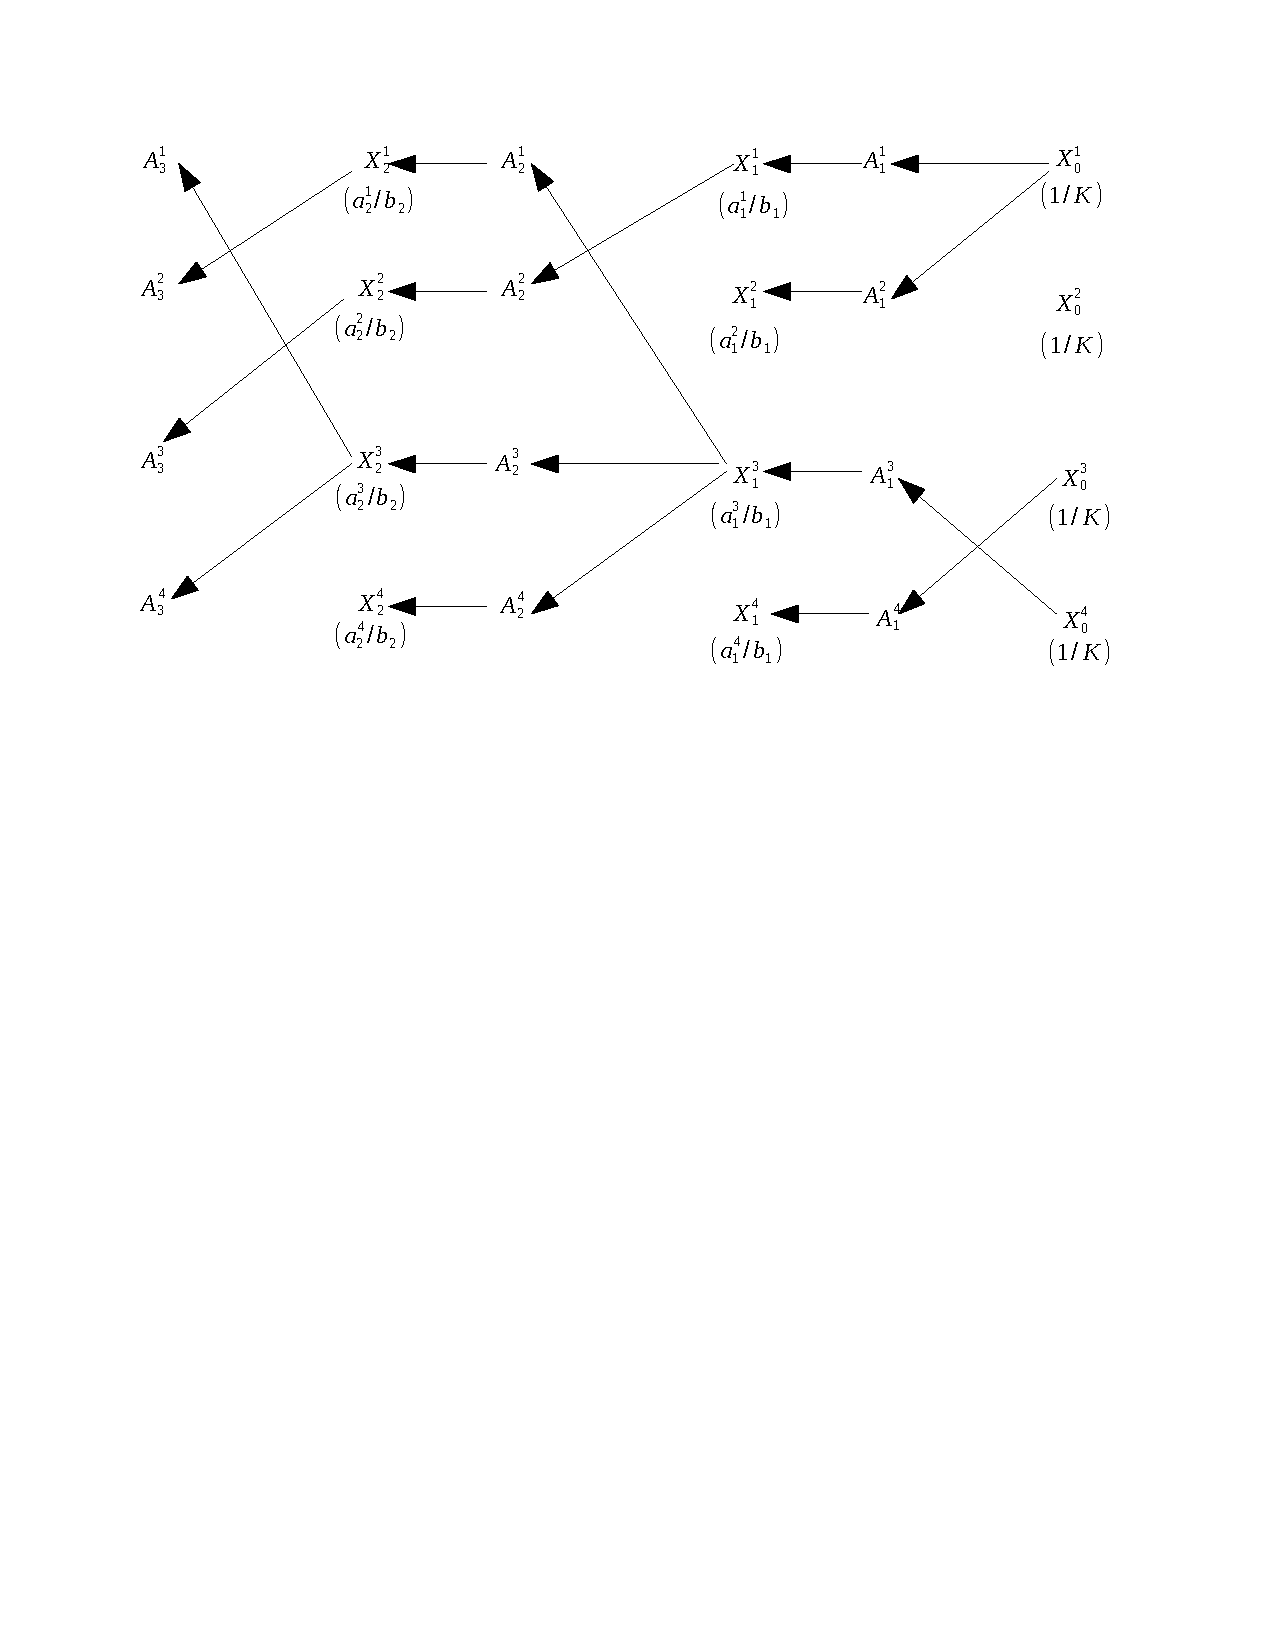
\includegraphics[width=\linewidth, trim=2cm 16cm 2.5cm 2cm, clip]{AnandsEstimator.pdf}
  \caption{A possible realization of the re-sampling procedure. $n =
    3$, $K = 4$. A number in a parenthesis indicates the probability
    of the unit vector above it being chosen to the next step.}
  \label{fig:AnandsEstimator}
\end{figure}
The difficulty with brute-force simulation and estimation is that,
when $n$ is large, the variance of $|\Pi_{n, 1} X_0|^\alpha$
is very large too, resulting in uselessly inaccurate estimations. One
approach of variance reduction is re-sampling. We divide the
estimation of $\Lambda(\alpha)$ into $n$ steps and we are prepared to
simulate $K$ realizations of $A_n, \dots, A_1$ and $X_0$. For
convenience, let
\begin{eqnarray*}
  M_n &=& \Pi_{n, 1} X_0 \\
  X_n &=& {M_n \over |M_n|}
\end{eqnarray*}
We can write
\begin{eqnarray*}
  M_n &=& A_n X_{n - 1} |M_{n - 1}| \\
  &=& A_n X_{n - 1} |A_{n-1} X_{n-2}| \cdot |M_{n-2}| \\
  &=& \cdots \\
  |M_n|^\alpha &=& \prod_{i=1}^n |A_i X_{i-1}|^\alpha
\end{eqnarray*}
With $K$ realizations of $A_n, \dots, A_1$ and $X_0$, a brute-force
estimator of ${1 \over n} \log(\E |M_n|^\alpha)$ can be
\[
{1 \over n} \log \left(
  {1 \over K} \sum_{l=1}^K \prod_{i=1}^n |A_i^l X^l_{i-1}|^\alpha
\right)
\]
where $A_i^l$ denotes the $l$-th realization of $A_i$ and
$X^l_{i-1} = A_{i-1}^l X^l_{i-2}/|A_{i-1}^l X^l_{i-2}|$. To reduce the
variance of the estimator, we introduce a re-sampling procedure:
\begin{equation}
  \label{eq:AnandsEstimator}
  \mathscr E_\alpha =
  {1 \over n}
  \sum_{i=1}^n \log \left(
    {1 \over K}\sum_{l=1}^K |A_i^l X^{w_{l, i-1}}_{i-1}|^\alpha
  \right)
\end{equation}
where the random variable $w_{l, i-1}$ has conditional distribution
\begin{eqnarray*}
  \P(w_{l, i-1} = j | w_{1, i-2}, \dots, w_{K, i-2}) &=& {a^j_{i-1} \over b_{i-1}} \\
  a_{i-1}^j &=& |A_{i-1}^j X_{i-2}^{w_{j, i-2}}|^\alpha \\
  b_{i-1} &=& \sum_{l=1}^K a_{i-1}^l
\end{eqnarray*}
\begin{theorem}
  \[
  \E \left\{
    \sum_{i=1}^n \log \left(
      {1 \over K}\sum_{l=1}^K |A_i^l X^{w_{l, i-1}}_{i-1}|^\alpha
    \right)
  \right\} = \log \left(
    \E |\Pi_{n, 1} X_0|^\alpha
  \right)
  \]
\end{theorem}
Figure \ref{fig:AnandsEstimator} shows a possible realization of the
resampling procedure and algorithm \ref{alg:Lambda_estimation}
outlines an implementation of $\mathscr E_\alpha$. We take
$|\cdot|$ as the max norm.
For an GARCH($p, q$) processes, the $A_i$ matrices have dimension
$d \times d$, where $d = p + q - 1$, and the $X_i$ are $d$-dimensional
unit vectors. 
\begin{algorithm}[H]
  \caption{Algorithm for estimating
    $\Lambda(\alpha) = \lim_{n \to \infty} {1 \over n} \log\left(\E |\Pi_{n, 1}|^\alpha \right)$}
  \label{alg:Lambda_estimation}
  \begin{algorithmic}
    \Procedure{$\mathscr E_\alpha$}{$n, K$}
    \State Define $K$ $d$-dimensional vectors $X^1, \dots, X^K$
    \State Define $K$ $d$-dimensional vectors $Y^1, \dots, Y^K$
    \State Define $K$-dimensional vector $a \gets (1, 1, \dots, 1)$
    \Comment{Initialize the weights}
    \For {$i$ from 1 to $K$}\Comment{Generate initial unit vectors}
    \For {$k$ from 1 to $d$}
    \State Generate a $U(0, 1)$ variable $U$
    \State $X^i(k) \gets U$ \Comment{$X^i(k)$ is the $k$-th component of $X^i$}
    \EndFor
    \State $X^i \gets X^i/|X^i|$
    \EndFor

    $\Lambda \gets 0$

    \For{$j$ from 1 to $n$}

    \State Define $K$-dimensional vector $Q$
    \State $Q(k) \gets \sum_{i=1}^k a(i)$ for all $k=1,2,\dots, K$
    \State Generate $K$ $d \times d$ random matrices $A^1, \dots, A^K$.

    \For{$k$ from 1 to $K$}
    \State Generate a $U(0, Q(K))$ variable $U$.
    \State $l \gets \min\{1 \leq i \leq K: Q(i) > U\}$
    \State $Y^k \gets A^k X^l$
    \State $a(k) \gets |Y^k|$
    \State $Y^k \gets Y^k/a(k)$
    \State $a(k) \gets a(k)^\alpha$
    \EndFor

    \State For all $k=1,\dots,K$, $X^k \gets Y^k$
    \State $\Lambda \gets \Lambda + {1 \over n}\log\left( { Q(K) \over K} \right)$
    \EndFor
    \State $\Lambda \gets \Lambda + {1 \over n}\log\left[ {1 \over K}\sum_{k=1}^K a(k) \right]$

    \Return $\Lambda$
    \EndProcedure
  \end{algorithmic}
\end{algorithm}

%% \ifestimation
\section{Sampling from the shifted conditional distribution}
While the Radon-Nikodym derivative of the shifted conditional
probability measure with respect to the original measure is given by
\eqref{eq:sampling}, the procedure of sampling from the shifted
conditional distribution is not trivial. For this purpose, we first
sample from the original distribution, and obtain an iid sample
$\hat Z_1^2, \hat Z_2^2, \dots, \hat Z_n^2$. This allows us to
compute, empirically, the shifted conditional distribution function
and its inverse:
\begin{eqnarray*}
  F_\xi(a, x) =
  \P^\xi(Z_t^2 \leq a | X_{t-1} = x) 
  &=&
  \int_0^a {
    |A(w)|^\xi r_\xi(A(w) \cdot x)
    \over
    r_\xi(x)
  } f_{Z^2}(w) dw \\
  \hat F_\xi(a, x)
  &=&
  \sum_{i=1}^n {
    |A(\hat Z_i^2)|^\xi r_\xi(A(\hat Z_i^2) \cdot x)
    \over
    r_\xi(x)
  } \1{\hat Z_i^2 \leq a } f_{Z^2}(\hat Z_i^2)
\end{eqnarray*}
where $f_{Z^2}$ denotes the original distribution of
$Z^2 \sim Z_i^2, i=1,2,\dots$ and  $\hat F_\xi(a, x)$ denotes the
empirical conditional distribution function. Now that $\hat F_\xi(a,
x)$ can be computed, one can also compute $\hat F_\xi^{-1}(p, x)$. Let
\[
k = \left\{
  \begin{array}{ll}
    \max\{1 \leq i \leq n: F_\xi(\hat Z_{(i)}^2, x) \leq p\} &
    \hat F_\xi(\hat Z_{(1)}, x) \leq p \\
    0 & \text{ otherwise }
  \end{array}
\right.
\]
where $\hat Z_{(1)}^2 < \cdots < \hat Z_{(i-1)}^2 < \hat Z_{(i)}^2 < \cdots <
\hat Z_{(n)}^2$ denote the order statistics of the sample $\{\hat
Z_{i}^2\}_{i=1}^n$. Then we assign
\[
\hat F_\xi^{-1}(p, x)
= \left\{
  \begin{array}{ll}
    \hat Z_{(1)}^2 + \left[p - \hat F_\xi(\hat Z_{(1)}^2, x)\right] {
      \hat Z_{(2)}^2 - \hat Z_{(1)}^2
      \over
      \hat F_\xi(\hat Z_{(2)}^2, x) - \hat F_\xi(\hat Z_{(1)}^2, x)
    } & k = 0 \\
    \hat Z_{(k)}^2 + \left[p - \hat F_\xi(\hat Z_{(k)}^2, x)\right] \cdot {
      \hat Z_{(k+1)} - \hat Z_{(k)}
      \over
      \hat F_\xi(Z_{(k+1)}, x) - \hat F_\xi(Z_{(k)}, x)
    } & 1 \leq k < n \\
    \hat Z_{(n)}^2 + \left[p - \hat F_\xi(\hat Z_{(n)}^2, x)\right] {
      \hat Z_{(n)}^2 - \hat Z_{(n-1)}^2
      \over
      \hat F_\xi(\hat Z_{(n)}^2, x) - F_\xi(\hat Z_{(n-1)}^2, x)
    } & k = n
  \end{array}
\right.
\]
In plain words, if $\hat F_\xi(\hat Z_{(1)}^2, x) < p < \hat F_\xi(\hat
Z_{(n)}^2, x)$, we interpolate the empirical quantile function; if
$p < \hat F_\xi(\hat Z_{(1)}^2, x)$, we compute $\hat F_\xi^{-1}(p,
x)$ by approximating the probability density function between
$\hat F_\xi^{-1}(p, x)$ and $\hat Z_{(1)}^2$ with ${\hat Z_{(2)}^2 - \hat
  Z_{(1)}^2 \over \hat F_\xi(\hat Z_{(2)}^2, x) - \hat F_\xi(\hat
  Z_{(1)}^2, x)}$; if $p > \hat F_\xi(\hat Z_{(n)}^2, x)$, $\hat F_\xi^{-1}(p,
x)$ is similarly approximated as in the previous case.

With a procedure to compute $\hat F^{-1}_\xi(p, x)$, we can sample
from the conditional distribution $\hat F_\xi(\cdot, x)$ by first
generating a $U(0, 1)$ random variable $U$ and giving
$\hat F^{-1}_\xi(U, x)$ as the desired random variable.

\section{An example: The GARCH(2,1) process}
As an example of the algorithms described in the previous sections, we
consider GARCH(2,1) processes. In this particular case we have
\begin{eqnarray*}
  \sigma_t^2 &=& \omega + \alpha_1 R_{t-1}^2 + \alpha_2 R_{t-2}^2 +
  \beta_1 \sigma_{t-1}^2
\end{eqnarray*}
Or in matrix forms
\begin{eqnarray}
  \begin{pmatrix}
    \sigma_t^2 \\
    R_{t-1}^2
  \end{pmatrix}
  &=&
  \begin{pmatrix}
  \alpha_1 Z_{t-1}^2 + \beta_1 & \alpha_2 \\
  Z_{t-1}^2 & 0
  \end{pmatrix}
  \begin{pmatrix}
    \sigma_{t-1}^2 \\
    R_{t-2}^2
  \end{pmatrix}
  +
  \begin{pmatrix}
    \omega \\
    0
  \end{pmatrix}
  \label{eq:garch21} \\
  V_t &=& A_t V_{t-1} + B \nonumber
\end{eqnarray}
where $R_t$ is the $t$-th observation of the sequence in question and
$Z_t$ are i.i.d $N(0,1)$ random variables. In the following we check
the conditions of theorem \ref{thrm:efficiency} against this process. 

As mentioned in remark \ref{remark:fhrtgh}, Bollerslev's assumption
$\alpha_1 + \alpha_2 + \beta_1 < 1$ implies that the top Lyapunov
exponent associated with the model \eqref{eq:garch21} is
negative. In the following we check the condition of theorem
\ref{thrm:efficiency} with regard to this model.

\begin{lemma}
  \label{lemma:frth}
  Assume $Z_t$ are i.i.d $N(0,1)$ random variables. Then
  $b^{1 - \xi/s} < e^\gamma$, where $b$ is defined in lemma
  \ref{lemma:2}, $\xi$ is the tail index of the stationary
  distribution of the markov chain $V_t$ as defined by
  \eqref{eq:garch21} and $\gamma$ is the top Lyapunov
  exponent of the matrices $A_t$ in \eqref{eq:garch21}.
\end{lemma}
\begin{proof}
First of all, we note $s$ of condition (I), hypothesis \ref{hypo:1}
can be arbitrarily large since $Z_t$ are i.i.d $N(0,1)$ random
variables. Therefore $b^{1 - \xi/s} < e^\gamma$ holds if $b <
e^\gamma$. To show the latter inequality holds, it suffices to show
there exists $\theta \in (0, \xi)$ such that $b_\theta < e^\gamma$,
where $b_\theta$ is defined in lemma \ref{lemma:1}.

If $\theta < 1$, $b_\theta$ is given by \eqref{eq:kpofew}:
\[
b_\theta = 
\lambda(\theta)
\left[
  1 + 
  {|B|^\theta r_{\theta}(\tilde B) 
    \over
    \lambda(\theta) M_{\theta} \underline r_\theta
  }
  \right]
\]
Because $M_\theta$ can be chosen arbitrarily large,
$b_\theta < e^\gamma$ holds if $\lambda(\theta) < e^\gamma$, or
equivalently $\log(\lambda(\theta)) < \gamma$.
Applying theorem 2 of Hennion \cite{hennion:1997} gives, for
an arbitrary fixed $\epsilon > 0$, there exists $N > T$ such that for
all $n > N$, ${1 \over n} \log \|\Pi_{n,1}\| < \gamma + \epsilon$.
This implies
\begin{equation*}
  {1 \over n} \log\left(
  \E \|\Pi_{n,1} \|^\theta
  \right)
  <
  \theta (\gamma + \epsilon)
  \]
  Thus
  \[
  \log(\lambda(\theta))
  =
  \lim_{n \to \infty} {1 \over n} \log\left(
  \E \|\Pi_{n,1} \|^\theta
  \right)
  <
  \theta (\gamma + \epsilon)
\end{equation*}
Thus, if $\theta$ is chosen such that
$0 < \theta < {\gamma \over \gamma + \epsilon} < 1$,
we have $b_\theta < e^\gamma$. The proof is complete.
\end{proof}

\subsection{Evaluation of the right eigenfunction}
Recall that, for $0 < \theta < \xi$, the right eigenfunction
$r_\theta(\cdot)$ corresponding to eigenvalue $\lambda(\theta)$ of the
operator $\mathscr P^\theta$ defined in \eqref{eq:trhyh} satisfies
\begin{eqnarray}
  \label{eq:trhj}
  \E \left[
    |A x|^\theta r_\theta(A \cdotp x)
    \right]
  &=&
  \mathscr P^\theta r_\theta(x) = \lambda(\theta) r_\theta(x)
\end{eqnarray}
In the following we take $|\cdot|$ as the Euclidean norm. Then $x$
can be written as $x = (\cos w, \sin w)^\top$, $w \in (0, \pi/2)$ and
\begin{eqnarray*}
  A x &=&
  \begin{pmatrix}
    \alpha_2 \sin w + (Z_t^2 \alpha_1 + \beta_1) \cos w \\
    Z^2 \cos w
  \end{pmatrix}
\end{eqnarray*}
Let $A \cdot x = (\cos \varphi, \sin\varphi)^\top$. Then
\begin{eqnarray}
  Z_t^2 &=&
  {\tan\varphi (\alpha_2 \sin w + \beta_1 \cos w)
    \over
    \cos w (1- \alpha_1 \tan\varphi)
  } \label{eq:rthy} \\
  {d Z_{t}^2 \over d\varphi}
  &=&
  {
    (\alpha_2 \sin w + \beta_1 \cos w) \sec^2\varphi
    \over
    \cos w (1 - \alpha_1 \tan\varphi)^2
  } \nonumber
\end{eqnarray}
Using \eqref{eq:rthy} we can write
\[
|A x|^{\theta}
=
(\alpha_2^2 + \beta_1^2)^{\theta/2}
{
  \sin^\theta\left(
  w + \arctan{\beta_1 \over \alpha_2}
  \right)
  \over
  \cos^\theta\varphi (1 - \alpha_1 \tan\varphi)^\theta
}
\]
It also becomes clear from \eqref{eq:rthy}
\[
x \in \left\{(\cos w, \sin w)^\top:
w \in \Omega = \left[0, \arctan{1 \over \alpha_1}\right)
\right\}
\quad
t = 0,1,2,\dots
\]
Define
\[
h_\theta(w): w \in \Omega \to (\underline r_\theta, \bar r_\theta)
\ni r_\theta((\cos w, \sin w)^\top)
\]
Then \eqref{eq:trhj} can be rewritten as
\begin{eqnarray}
  \lambda(\theta) h_\theta(w)
  &=&
\int_\Omega (\alpha_2^2 + \beta_1^2)^{\theta/2} {
  \sin^\theta\left(
  w + \arctan{\beta_1 \over \alpha_2}
  \right)
  \over
  \cos^\theta\varphi (1 - \alpha_1 \tan\varphi)^\theta
}
f_{\chi^2}\left[
{\tan\varphi (\alpha_2 \sin w + \beta_1 \cos w)
  \over
  \cos w (1- \alpha_1 \tan\varphi)
} \right] \times \nonumber\\
&&
h_\theta(\varphi)
{
  (\alpha_2 \sin w + \beta_1 \cos w) \sec^2\varphi
  \over
  \cos w (1 - \alpha_1 \tan\varphi)^2
}
d\varphi \nonumber \\
\lambda(\theta) h_\theta(w)
&=&
\int_\Omega H_\theta(w, \varphi) h_\theta(\varphi) d\varphi
\end{eqnarray}
where $f_{\chi^2}(\cdot)$ is the probability density function of the
$\chi^2$ distribution; the function $H_\theta(w, \varphi)$ has been defined
for convenience.
We may approximate the last integral with a sum and the function
$h_\theta(\cdot)$ with a vector:
\[
\lambda(\theta) h_\theta(i \Delta_n)
\approx
\Delta_n \sum_{j=0}^{n-1} H_\theta(i \Delta_n, j \Delta_n) h_\theta(j \Delta_n)
\]
where $\Delta_n = {\arctan(1/\alpha_1) \over n}$.
Thus $\lambda(\theta)$ can be found as the spectral radius of 
matrix $\Delta_n H_\theta(i \Delta_n, j \Delta_n)$ and 
$\{h_\theta(i \Delta_n)\}_ {i=1,2,\dots, n}$ as the associated
eigenvector (cf. Collamore and Mentemeier
\cite{collamore:mentemeier:2016}, lemma 2.2).

\subsection{Simulaton and Results}
In this section we describe the implementation of the estimator
$\mathcal E_u$ when $V_t$ is a GARCH($2, 1$) process. In previous
sections we have shown that $\mathcal E_u$ is efficient for
GARCH($2, 1$) and described how the right eigenfunctions can be
approximately evaluated. It remains to choose the set
$\mathcal C = \{v \in \chi, |V_n| < M\}$.

For convenience, we take $\Theta = [\xi/4, 3\xi/4]$
(cf. \S\ref{sec:bound_to_C}).


% To estimate the 
% values of $\omega, \alpha_1, \alpha_2, \beta_1$, we use the ``fGarch''
% package of the ``R'' language. Its ``garchFit'' function provides
% routine to fit a specified type of model to a given series.
% The ``garchFit'' function provides 4 algorithms for maximum likelihood
% estimation of the parameters. We choose its default algorithm ``nlminb'',
% i.e. ``unconstrained and box-constrained optimization using PORT
% routines''. The ``fGarch'' package is developed and maintained by {\it
% Rmetrics} (https://www.rmetrics.org/).

  
% \subsubsection{S\&P 500}
% \begin{itemize}
% \item GARCH(1, 1)
%   When modeled as a GARCH(1, 1) process, the S\&P 500 return series
%   has the coefficients as shown in the following equation
%   \[
%   \sigma_t^2 = 0.15 R_{t-1}^2 + 0.72 \sigma_{t-1}^2 + 7.4 \times 10^{-6}
%   \]
%   The tail index of the stationary distribution of $\sigma_t^2$ is
%   estimated at 4.4465. On the other hand, the Hill estimator puts the
%   tail index of the inferred $\sigma_t^2$ at 4.3372.

% \item GARCH(2, 1)
%   When fitted to a GARCH(2, 1) process, the S\&P 500 return series has
%   the following model
%   %% 7.949678e-02, 8.765884e-02, 9.376992e-06
%   \[
%   \sigma_t^2 = 0.079 R_{t-1}^2 + 0.088 R_{t-2}^2 + 0.668 \sigma_{t-1}^2 + 9.4 \times 10^{-6}
%   \]
%   Using the proposed re-sampling algorithm, our estimate of the tail
%   index is $4.30026$. The values of $\Lambda(\alpha)$ in the
%   neighborhood of $\alpha = \xi$ is listed in table
%   \ref{tab:SP500_garch21_tail_index}.
%   \begin{table}[htb!]
%     \centering
%     \begin{tabular}{l|l|l|l||l|l|l|l}
%       $\alpha$ & $\Lambda(\alpha)$ & err. & rel. err. & $\alpha$ & $\Lambda(\alpha)$ & err. & rel. err. \\
%       \hline
%       0.1000 & -0.0186 & 0.0007 & 0.0378 & 3.1000 & -0.2020 & 0.2175 & 1.0766\\
%       0.2000 & -0.0366 & 0.0012 & 0.0329 & 3.2000 & -0.1921 & 0.2360 & 1.2286\\
%       0.3000 & -0.0539 & 0.0016 & 0.0293 & 3.3000 & -0.1829 & 0.2765 & 1.5116\\
%       0.4000 & -0.0706 & 0.0020 & 0.0281 & 3.4000 & -0.1705 & 0.3121 & 1.8308\\
%       0.5000 & -0.0866 & 0.0024 & 0.0279 & 3.5000 & -0.1595 & 0.3335 & 2.0914\\
%       0.6000 & -0.1018 & 0.0030 & 0.0299 & 3.6000 & -0.1458 & 0.3665 & 2.5140\\
%       0.7000 & -0.1163 & 0.0045 & 0.0387 & 3.7000 & -0.1264 & 0.4249 & 3.3627\\
%       0.8000 & -0.1301 & 0.0059 & 0.0456 & 3.8000 & -0.1165 & 0.4285 & 3.6778\\
%       0.9000 & -0.1432 & 0.0083 & 0.0581 & 3.9000 & -0.0996 & 0.5233 & 5.2545\\
%       1.0000 & -0.1552 & 0.0104 & 0.0668 & 4.0000 & -0.0819 & 0.5479 & 6.6896\\
%       1.1000 & -0.1666 & 0.0137 & 0.0825 & 4.1000 & -0.0653 & 0.5806 & 8.8930\\
%       1.2000 & -0.1771 & 0.0168 & 0.0947 & 4.2000 & -0.0403 & 0.7173 & 17.8196\\
%       1.3000 & -0.1867 & 0.0206 & 0.1105 & 4.3000 & -0.0365 & 0.6749 & 18.5091\\
%       1.4000 & -0.1958 & 0.0246 & 0.1255 & 4.4000 & -0.0055 & 0.7390 & 135.2172\\
%       1.5000 & -0.2038 & 0.0299 & 0.1467 & 4.5000 & 0.0186 & 0.8443 & 45.4573\\
%       1.6000 & -0.2107 & 0.0353 & 0.1675 & 4.6000 & 0.0267 & 0.7493 & 28.0286\\
%       1.7000 & -0.2169 & 0.0398 & 0.1836 & 4.7000 & 0.0614 & 0.9068 & 14.7576\\
%       1.8000 & -0.2226 & 0.0467 & 0.2099 & 4.8000 & 0.0867 & 0.9380 & 10.8220\\
%       1.9000 & -0.2271 & 0.0543 & 0.2392 & 4.9000 & 0.0973 & 0.8703 & 8.9467\\
%       2.0000 & -0.2299 & 0.0607 & 0.2642 & 5.0000 & 0.1275 & 0.9424 & 7.3918\\
%       2.1000 & -0.2320 & 0.0685 & 0.2953 & 5.1000 & 0.1618 & 1.0582 & 6.5403\\
%       2.2000 & -0.2344 & 0.0760 & 0.3244 & 5.2000 & 0.1721 & 0.8950 & 5.2004\\
%       2.3000 & -0.2343 & 0.0903 & 0.3856 & 5.3000 & 0.2081 & 0.9849 & 4.7334\\
%       2.4000 & -0.2341 & 0.0994 & 0.4246 & 5.4000 & 0.2411 & 1.0852 & 4.5009\\
%       2.5000 & -0.2320 & 0.1106 & 0.4767 & 5.5000 & 0.2378 & 0.9362 & 3.9375\\
%       2.6000 & -0.2291 & 0.1273 & 0.5555 & 5.6000 & 0.2605 & 0.9805 & 3.7635\\
%       2.7000 & -0.2273 & 0.1365 & 0.6007 & 5.7000 & 0.3306 & 1.0445 & 3.1596\\
%       2.8000 & -0.2214 & 0.1595 & 0.7205 & 5.8000 & 0.3301 & 1.0014 & 3.0333\\
%       2.9000 & -0.2143 & 0.1667 & 0.7781 & 5.9000 & 0.3562 & 1.0427 & 2.9270\\
%       3.0000 & -0.2075 & 0.2034 & 0.9804 & 6.0000 & 0.3891 & 0.9544 & 2.4525
%     \end{tabular}
%     \caption{SP500: $\Lambda(\alpha)$ around $\alpha = \xi$. N = 400, K = 40000}
%     \label{tab:SP500_garch21_tail_index}
%   \end{table}

%   \begin{minipage}{0.5\linewidth}
%     \centering
%     $\Lambda(\alpha)$
%     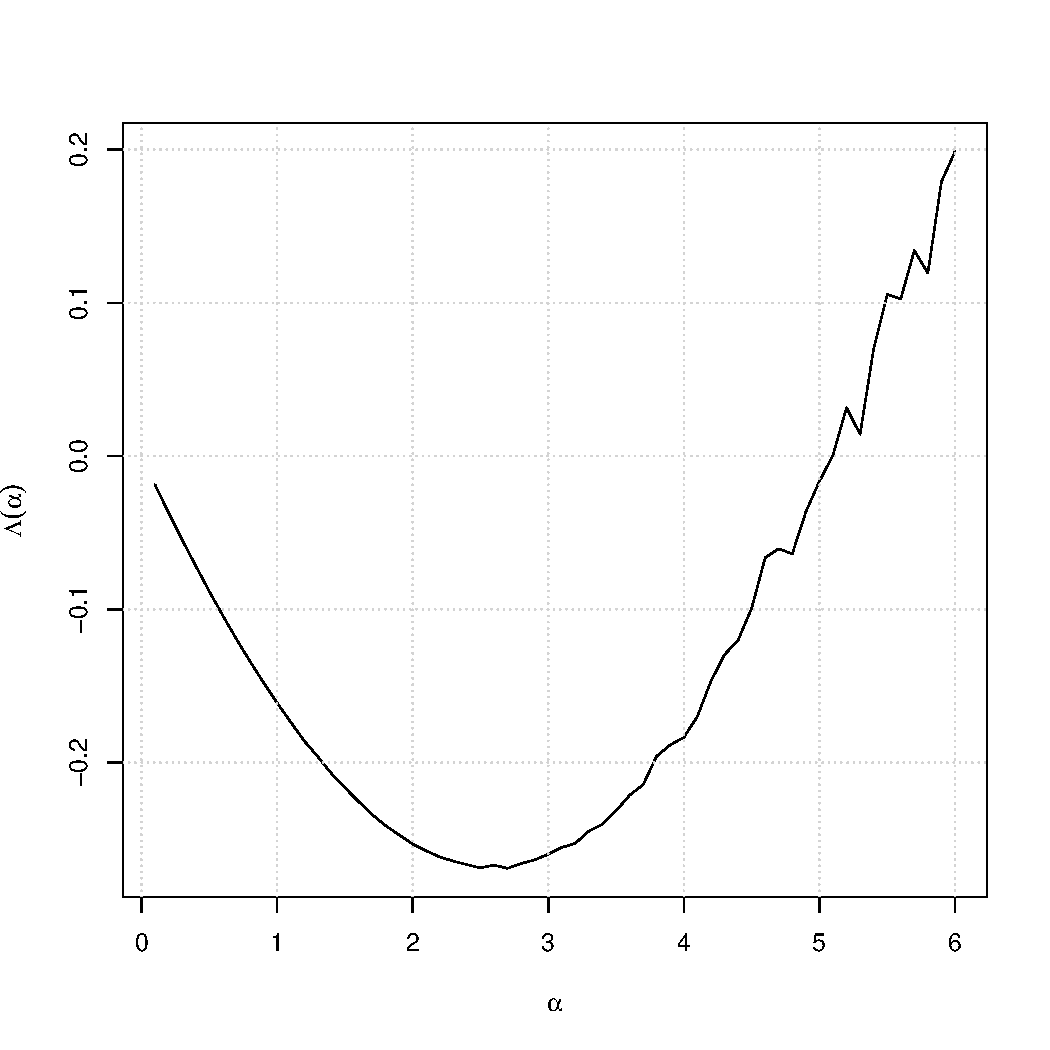
\includegraphics[width=\textwidth]{SP500_xi.pdf}
%   \end{minipage}\hfill
%   \begin{minipage}{0.5\linewidth}
%     \centering
%     $r_\xi(x)$ corresponding to $\xi$
%     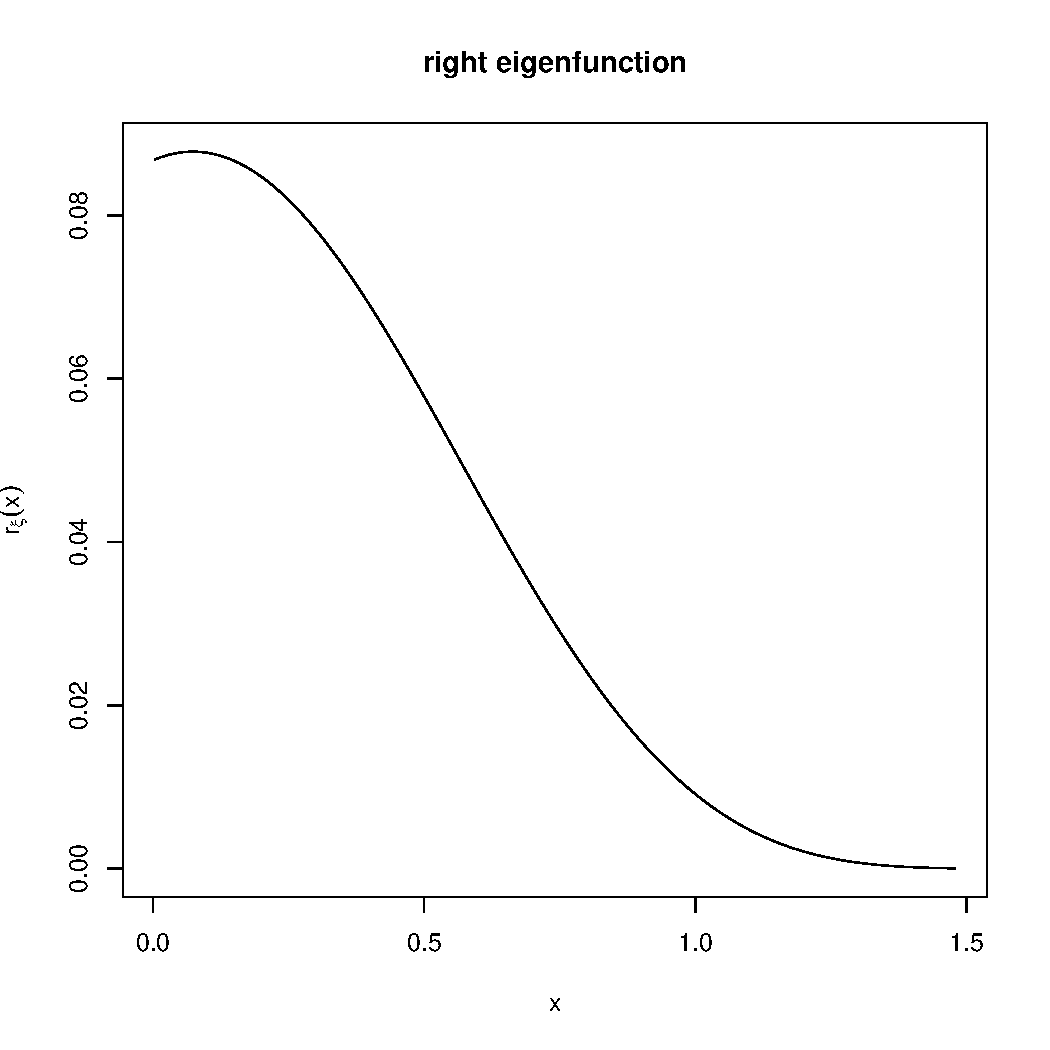
\includegraphics[width=\textwidth]{SP500_r.pdf}
%   \end{minipage}
% \end{itemize}

% \subsubsection{DAX}
% \begin{itemize}
% \item GARCH(1, 1)
%   When modeled as a GARCH(1, 1) process, the DAX return series
%   has the coefficients as shown in the following equation
%   \[
%   \sigma_t^2 = 0.06 R_{t-1}^2 + 0.92 \sigma_{t-1}^2 + 3.1 \times 10^{-6}
%   \]
%   The tail index of the stationary distribution of $\sigma_t^2$ is
%   estimated at 6.4269. The Hill estimator of this
%   sequence is computed at 6.6020.

% \item GARCH(2, 1)
%   When fitted to a GARCH(2, 1) process, the DAX return series has the following model
%   \[
%   \sigma_t^2 = 0.027 R_{t-1}^2 + 0.042 R_{t-2}^2 + 0.897 \sigma_{t-1}^2 + 4.0 \times 10^{-6}
%   \]
%   The algorithm with its current implementation has difficulty to
%   estimate $\Lambda(\alpha)$ as $\alpha$ becomes large. This is shown
%   in the figure below:
%   \begin{figure}[htb!]
%     \centering
%     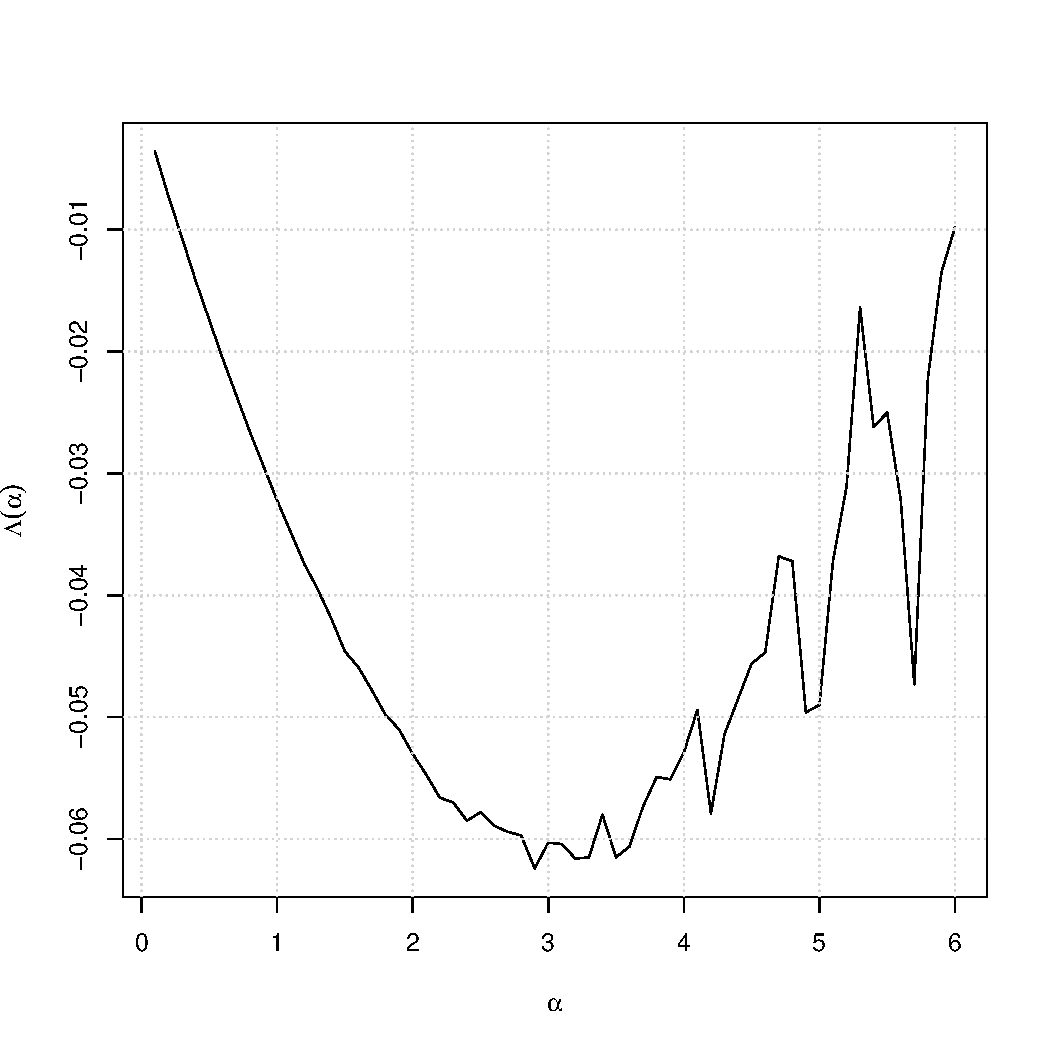
\includegraphics[width=\textwidth]{DAX_xi.pdf}
%     \caption{$\Lambda(\alpha)$ estimates for DAX}
%     \label{fig:DAX_garch21_tailindex}
%   \end{figure}
%   The estimated values of $\Lambda(\alpha)$ are listed table \ref{tab:DAX_garch21_tail_index}.
%     \begin{table}[htb!]
%     \centering
%     \begin{tabular}{l|l|l|l||l|l|l|l}
%       $\alpha$ & $\Lambda(\alpha)$ & err. & rel. err. & $\alpha$ & $\Lambda(\alpha)$ & err. & rel. err. \\
%       \hline
%       0.1000 & -0.0036 & 0.0009 & 0.2535 & 3.1000 & -0.0604 & 0.2027 & 3.3558 \\
%       0.2000 & -0.0073 & 0.0017 & 0.2340 & 3.2000 & -0.0616 & 0.2585 & 4.1940 \\
%       0.3000 & -0.0107 & 0.0020 & 0.1903 & 3.3000 & -0.0615 & 0.2669 & 4.3419 \\
%       0.4000 & -0.0142 & 0.0025 & 0.1763 & 3.4000 & -0.0580 & 0.3232 & 5.5729 \\
%       0.5000 & -0.0174 & 0.0027 & 0.1531 & 3.5000 & -0.0615 & 0.3719 & 6.0467 \\
%       0.6000 & -0.0206 & 0.0030 & 0.1445 & 3.6000 & -0.0606 & 0.3794 & 6.2604 \\
%       0.7000 & -0.0236 & 0.0038 & 0.1624 & 3.7000 & -0.0573 & 0.4485 & 7.8213 \\
%       0.8000 & -0.0266 & 0.0050 & 0.1884 & 3.8000 & -0.0549 & 0.5345 & 9.7438 \\
%       0.9000 & -0.0294 & 0.0073 & 0.2469 & 3.9000 & -0.0551 & 0.5655 & 10.2685 \\
%       1.0000 & -0.0322 & 0.0089 & 0.2774 & 4.0000 & -0.0529 & 0.6865 & 12.9826 \\
%       1.1000 & -0.0348 & 0.0109 & 0.3127 & 4.1000 & -0.0494 & 0.7077 & 14.3304 \\
%       1.2000 & -0.0374 & 0.0146 & 0.3904 & 4.2000 & -0.0579 & 0.7418 & 12.8088 \\
%       1.3000 & -0.0395 & 0.0178 & 0.4515 & 4.3000 & -0.0514 & 0.8021 & 15.6075 \\
%       1.4000 & -0.0419 & 0.0218 & 0.5210 & 4.4000 & -0.0485 & 0.9369 & 19.3079 \\
%       1.5000 & -0.0446 & 0.0260 & 0.5821 & 4.5000 & -0.0456 & 0.9525 & 20.8980 \\
%       1.6000 & -0.0459 & 0.0304 & 0.6634 & 4.6000 & -0.0447 & 1.0402 & 23.2610 \\
%       1.7000 & -0.0478 & 0.0356 & 0.7443 & 4.7000 & -0.0368 & 1.0678 & 28.9796 \\
%       1.8000 & -0.0498 & 0.0421 & 0.8452 & 4.8000 & -0.0372 & 1.1068 & 29.7502 \\
%       1.9000 & -0.0510 & 0.0482 & 0.9443 & 4.9000 & -0.0496 & 1.1848 & 23.8698 \\
%       2.0000 & -0.0530 & 0.0543 & 1.0236 & 5.0000 & -0.0490 & 1.1304 & 23.0528 \\
%       2.1000 & -0.0547 & 0.0650 & 1.1877 & 5.1000 & -0.0372 & 1.3674 & 36.7623 \\
%       2.2000 & -0.0566 & 0.0713 & 1.2610 & 5.2000 & -0.0311 & 1.3533 & 43.5658 \\
%       2.3000 & -0.0570 & 0.0820 & 1.4393 & 5.3000 & -0.0164 & 1.3191 & 80.2003 \\
%       2.4000 & -0.0585 & 0.0914 & 1.5631 & 5.4000 & -0.0262 & 1.4752 & 56.2897 \\
%       2.5000 & -0.0578 & 0.1070 & 1.8514 & 5.5000 & -0.0250 & 1.3379 & 53.5797 \\
%       2.6000 & -0.0589 & 0.1163 & 1.9759 & 5.6000 & -0.0322 & 1.4219 & 44.1810 \\
%       2.7000 & -0.0594 & 0.1302 & 2.1913 & 5.7000 & -0.0473 & 1.3915 & 29.4468 \\
%       2.8000 & -0.0597 & 0.1516 & 2.5405 & 5.8000 & -0.0222 & 1.6773 & 75.3996 \\
%       2.9000 & -0.0624 & 0.1663 & 2.6664 & 5.9000 & -0.0135 & 1.4893 & 110.0806 \\
%       3.0000 & -0.0603 & 0.1877 & 3.1148 & 6.0000 & -0.0098 & 1.5522 & 158.6270
%     \end{tabular}
%     \caption{DAX: $\Lambda(\alpha)$ around $\alpha = \xi$. N = 400, K = 40000}
%     \label{tab:DAX_garch21_tail_index}
%   \end{table}

% \end{itemize}



